% Time-stamp: <2023-04-15 17:33:11 A13258Q>
% Romain Lafarguette 2020, https://romainlafarguette.github.io/

%% ---------------------------------------------------------------------------
%% Preamble: Packages and Setup
%% ---------------------------------------------------------------------------
% Class 
\documentclass{beamer}

% Theme
\usetheme{Boadilla}
\usecolortheme{dolphin}
%\setbeamertemplate{headline}{} % Remove the top navigation bar

% Font and encoding
\usepackage[utf8]{inputenc} % Input font
\usepackage[T1]{fontenc} % Output font
\usepackage{lmodern} % Standard LateX font
\usefonttheme{serif} % Standard LateX font

% Maths 
\usepackage{amsfonts, amsmath, mathabx, bm, bbm} % Maths Fonts

% Graphics
\usepackage{graphicx} % Insert graphics
\usepackage{subfig} % Multiple figures in one graphic
\graphicspath{{/img}}

% Layout
\usepackage{changepage}

% Colors
\usepackage{xcolor}
\definecolor{imfblue}{RGB}{0,76,151} % Official IMF color
\setbeamercolor{title}{fg=imfblue}
\setbeamercolor{frametitle}{fg=imfblue}
\setbeamercolor{structure}{fg=imfblue}

% Tables
\usepackage{booktabs,rotating,multirow} % Tabular rules and other macros
%\usepackage{pdflscape,afterpage} % Landscape mode and afterpage
%\usepackage{threeparttable} % Split long tables
\usepackage[font=scriptsize,labelfont=scriptsize,labelfont={color=imfblue}]{caption}

% Import files
\usepackage{import}

% Appendix slides
\usepackage{appendixnumberbeamer} % Manage page numbers for appendix slides

% References
\usepackage{hyperref}

% A few macros: environments
\newenvironment{wideitemize}{\itemize\addtolength{\itemsep}{10pt}}{\enditemize}
\newenvironment{wideenumerate}{\enumerate\addtolength{\itemsep}{10pt}}{\endenumerate}

\newenvironment{extrawideitemize}{\itemize\addtolength{\itemsep}{30pt}}{\enditemize}
\newenvironment{extrawideenumerate}{\enumerate\addtolength{\itemsep}{30pt}}{\endenumerate}

% Remove navigation symbols and other superfluous elements
\setbeamertemplate{navigation symbols}{}
\beamertemplatenavigationsymbolsempty

%\setbeamertemplate{note page}[plain]
\hypersetup{pdfpagemode=UseNone} % don't show bookmarks on initial view
\setbeameroption{hide notes}

% Institute font
\setbeamerfont{institute}{size=\footnotesize}
\DeclareMathSizes{10}{9}{7}{5}

% Footnote without marker
\newcommand\blfootnote[1]{%
  \begingroup
  \renewcommand\thefootnote{}\footnote{#1}%
  \addtocounter{footnote}{-1}%
  \endgroup
}

%% ---------------------------------------------------------------------------
%% Title info
%% ---------------------------------------------------------------------------
\title[FXI Theory \& Practice]{Foreign Exchange Interventions \\ Theory and Practice}

\author[Lafarguette \& Raboun]{Romain Lafarguette, Ph.D. \and Amine Raboun, Ph.D.}
\institute[IMF STX]{Quants \& IMF External Experts\blfootnote{\scriptsize{\emph{This training material is the property of the IMF, any reuse requires IMF permission}}} \\
\begin{center}{\href{https://romainlafarguette.github.io/}{\textcolor{imfblue}{romainlafarguette.github.io/}} \hspace{0.3cm} \href{https://amineraboun.github.io/}{\textcolor{imfblue}{amineraboun.github.io/}}} \end{center} \vspace{-0.5cm}} 

\date[STI, 17 April 2023]{\footnotesize Singapore Training Institute, 17 April 2023}

\titlegraphic{\vspace{-0.6cm}
    \begin{figure}
    \centering
    \subfloat{{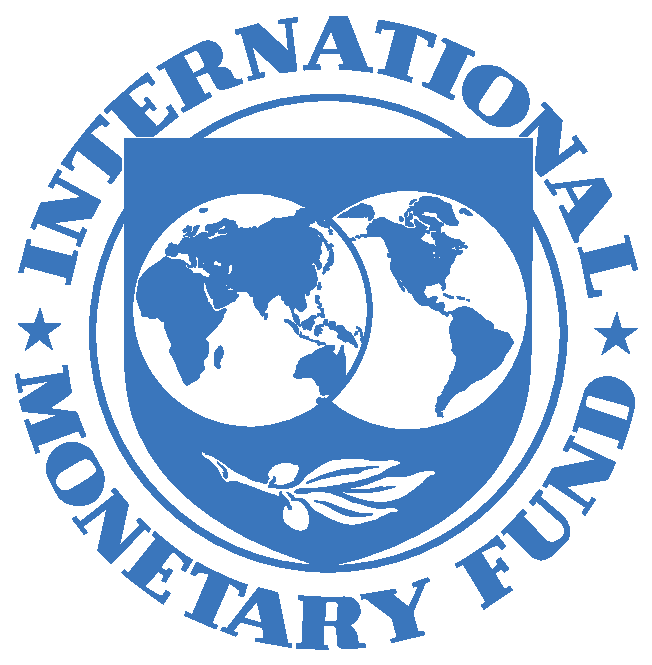
\includegraphics[width=2cm]{img/imf_logo}}}%
    \end{figure}}

% Slide between sections
\AtBeginSection[]
{
    \begin{frame}
        \tableofcontents[currentsection]
    \end{frame}
}

%% ---------------------------------------------------------------------------
%% Title slide
%% ---------------------------------------------------------------------------
\begin{document}

\begin{frame}
\maketitle
\end{frame}

\begin{frame}
  \frametitle{Resources}
  \begin{wideitemize}

  \item A textbook presentation of foreing exchange interventions can be found in Sarno and Taylor (2012): \href{https://www.cambridge.org/core/books/abs/economics-of-exchange-rates/official-intervention-in-the-foreign-exchange-market/539435B26391C092195233098F887850}{\beamergotobutton{The Economics of Exchange Rate}}
        
  \item The BIS publishes interesting papers reflecting BIS surveys conducted with central banks. For instance (2019): \href{https://www.bis.org/publ/bppdf/bispap104b-rh.pdf}{\beamergotobutton{FX Interventions: Goals, Strategies and Tactics}}
    
  \item A recent and quite comprehensive database on FX Interventions (2021), compiled by IMF colleagues: \href{https://www.imf.org/en/Publications/WP/Issues/2021/02/19/Foreign-Exchange-Intervention-A-Dataset}{\beamergotobutton{Foreign Exchange Interventions, A Dataset}}

  \item I am borrowing materials from Kathryn Dominguez, professor at U-Michigan, specialized on FX interventions: \href{http://www-personal.umich.edu/~kathrynd/index.html}{\beamergotobutton{Kathryn Dominguez Personal Webpage}}

  \item Popper (2022) provides a very complete literature review on FX Interventions \href{https://www.ssc.wisc.edu/~mchinn/Popper_FXI_apr22.pdf}{\beamergotobutton{Link, Popper 2022}}
    
  \end{wideitemize}
\end{frame}


%% ---------------------------------------------------------------------------
%% Conceptual Framework
%% ---------------------------------------------------------------------------
\section{Conceptual Framework}

\begin{frame}
  \frametitle{Definition of FX interventions}

  \begin{alertblock}{FX Interventions: Definition}
    Any official sale or purchase of foreign assets against domestic assets \textbf{in the foreign exchange market}    
  \end{alertblock}

  \begin{itemize}
  \item FXI are usually carried-out by the central bank, but can sometimes be under the responsibility of the Ministry of Finance (eg. \href{https://www.mof.go.jp/english/policy/international_policy/reference/feio/index.html}{\beamergotobutton{Link}})
  \item \emph{To simplify, in this presentation, we assume that domestic assets are in the domestic currency, while foreign assets are denominated in the foreign currency}
  \end{itemize}  
\end{frame}


\subsection{Goals and Intermediate Objectives}
\begin{frame}
  \frametitle{Goals and Intermediate Objectives}

  
  \begin{wideitemize}
  \item \textbf{Goals}: ultimate purpose of the FX intervention. Consistent with the monetary framework of the central bank 
    
    \begin{itemize}
    \item \emph{For instance, preserving financial stability}
    \end{itemize}
    
    \item \textbf{Intermediate objectives}: reach the goals via the operational framework of the central bank  
      \begin{itemize}
      \item \emph{For instance, mitigating FX daily volatility}
      \end{itemize}
      
  \end{wideitemize}
\end{frame}


\begin{frame}
  \frametitle{FXI Main Goals for Central Banks}

  \begin{itemize}
  \item \textbf{Price stability}
    \begin{itemize}
    \item When large exchange rate movements pass-through inflation, generating temporary shocks
    \end{itemize}
    \item \textbf{Financial stability}
      \begin{itemize}
      \item Calm "disorderly market conditions"
      \item Smooth capital flows and credit spillovers (impact on carry trade and excess returns)
      \item Alleviate FX funding shortage
      \item Reduce FX speculation
      \end{itemize}
    \item \textbf{Terms of trade}
      \begin{itemize}
      \item Support external competitiveness (especially in USD weakening phases)
      \item Smooth commodity prices      
      \end{itemize}
    \item \textbf{Building/managing FX reserves}
      \begin{itemize}
        \item \emph{In principle, without market impact}
        \end{itemize}
    \item Support fellow central banks in their exchange rate operations
  \end{itemize}
\end{frame}


\begin{frame}
\frametitle{Survey: FXI Main Goals for Central Banks}
\makebox[\linewidth]{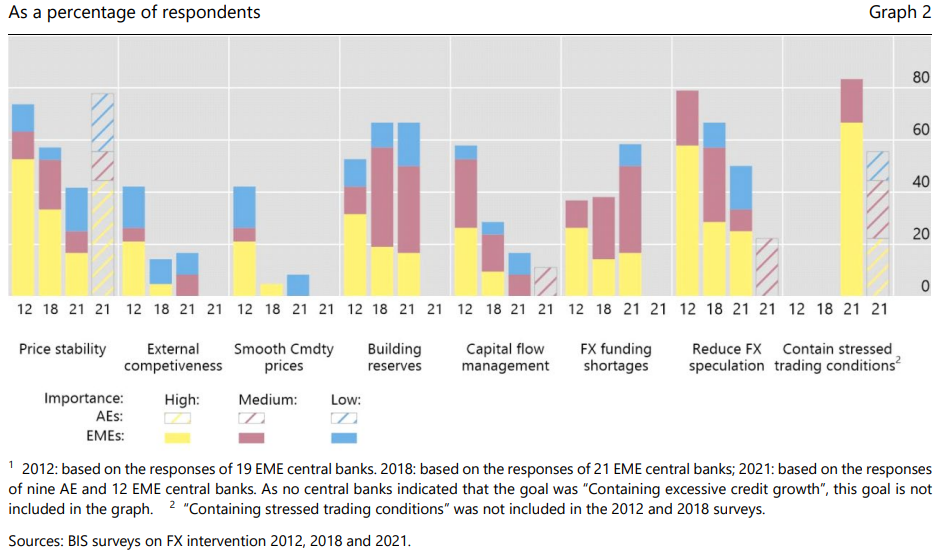
\includegraphics[width=0.7\paperwidth]{img/bis_fxi_goals.PNG}}
\medskip
\emph{Source: BIS 2021 \href{https://www.bis.org/publ/bppdf/bispap104b_rh.pdf}{\beamergotobutton{Link}}}
\end{frame}


\begin{frame}
  \frametitle{FXI Intermediate Objectives}
  \begin{wideitemize}
  \item \textbf{Limit exchange rate volatility}
    \begin{itemize}
    \item Even if the main goal is price stability, limiting FX volatility is important. Affect the price-setting behavior of firms; cause average imported inflation to rise. 
    \item Can derail the transmission of monetary policy
    \end{itemize}
    \item Provide liquidity to think market
    \item \textbf{Influence the level of exchange rate}
    \item Smooth the trend path of exchange rate
    \item Limit pressure caused by international investors

  \end{wideitemize}
\end{frame}


\begin{frame}
\frametitle{Survey: FXI Intermediate Objectives for Central Banks}
\makebox[\linewidth]{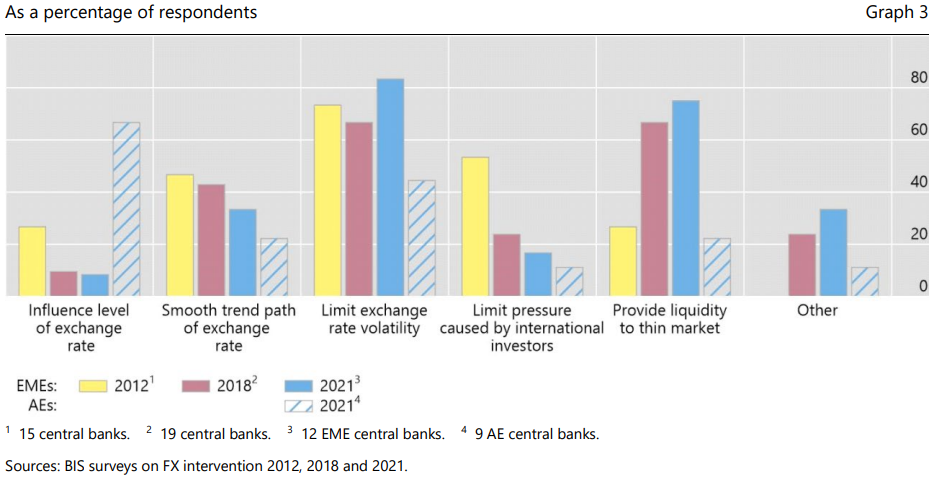
\includegraphics[width=0.7\paperwidth]{img/bis_intermediate_objectives.PNG}}
\medskip
\emph{Source: BIS 2021 \href{https://www.bis.org/publ/bppdf/bispap104b_rh.pdf}{\beamergotobutton{Link}}}
\end{frame}


\begin{frame}
  \frametitle{The Negative Impacts of FX Interventions}
  \begin{wideitemize}
    \item \textbf{Moral hazard} and encouragement of greater-risk taking
    \item \textbf{Negative effects on market development} (e.g. hampering the development of derivative markets by removing the need for currency hedge)
      \begin{itemize}
      \item which in turn increases the need for future FXI in the future...
      \end{itemize}
    \item Potential difficulties in balancing the \textbf{orderly functioning of local FX markets} while maintaining \textbf{openness to foreign investors}
    \item Possible inconsistencies between monetary policy and FXI, with complex interactions difficult to understand and communicate, which overall increase \textbf{policy uncertainty}
    \item \emph{Note that the risk-based intervention rule we will present during this course is solving some of these issues}
  \end{wideitemize}
\end{frame}


\subsection{Monetary Frameworks}

\begin{frame}
  \frametitle{FXI Interventions Should be Consistent with the Monetary Framework}

  
  \begin{wideitemize}
  \item \textbf{Inflation targeters and monetary base targeters} should parsimoniously use FX interventions for:
    \begin{itemize}
    \item Financial stability
      \begin{itemize}
      \item \emph{For instance, when domestic agents face severe currency mismatches on their balance sheet}
      \end{itemize}
    \item To ensure that the monetary objectives are reached
          \begin{itemize}
      \item \emph{For instance, when the pass-through of large  - and temporary - exchange rate movements threaten }
      \end{itemize}
    \end{itemize}
   
    \item \textbf{Hard-peg and currency board} regimes usually conduct FX operations via FX windows, at fixed exchange rate (the monetary policy objectives)

    \item \textbf{Crawling- and soft-peg} conduct infrequent FXI when the exchange rate deviates outside of the central bank tolerancce
      \begin{itemize}
      \item Often, conflict between \emph{de-jure} and \emph{de-facto} monetary objectives
      \end{itemize}
    \end{wideitemize}
\end{frame}


\begin{frame}
  \frametitle{Monetary Frameworks and Trilemma}
    \makebox[\linewidth]{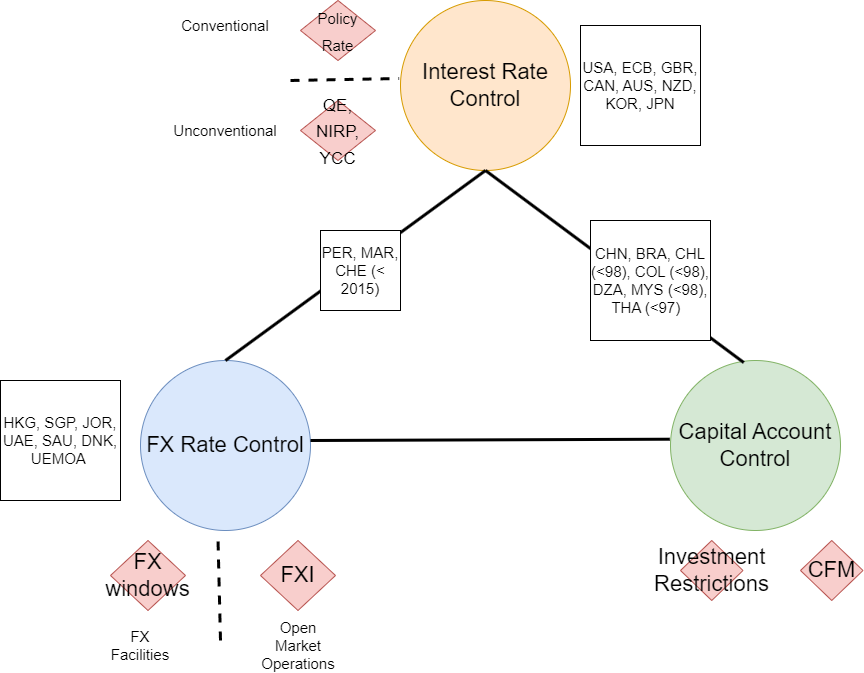
\includegraphics[height=0.8\paperheight]{img/Trilemma.png}}  
\end{frame}


\subsection{Types of FX Interventions}
\begin{frame}
  \frametitle{Types of FX Interventions}
  
  There are two types of foreign exchange interventions:\\
  \medskip

  \begin{enumerate}
  \item \textbf{Non-sterilized operations}
    \begin{itemize}
    \item Buy and sell foreign assets against banks' reserves at the central bank
    \item Increase or decrease the monetary base, and therefore impact the monetary stance
    \end{itemize}
  \item \textbf{Sterilized operations}
    \begin{itemize}
    \item Buy and sell foreign assets against banks' reserves at the central bank
    \item Sterilize the intervention by either (i) selling or purchasing home-currency assets or (ii) issuance of sterilization instruments 
    \item No impact on the monetary stance
    \end{itemize}
  \end{enumerate}
\end{frame}


\begin{frame}
\frametitle{Central Bank Balance Sheet}
    \makebox[\linewidth]{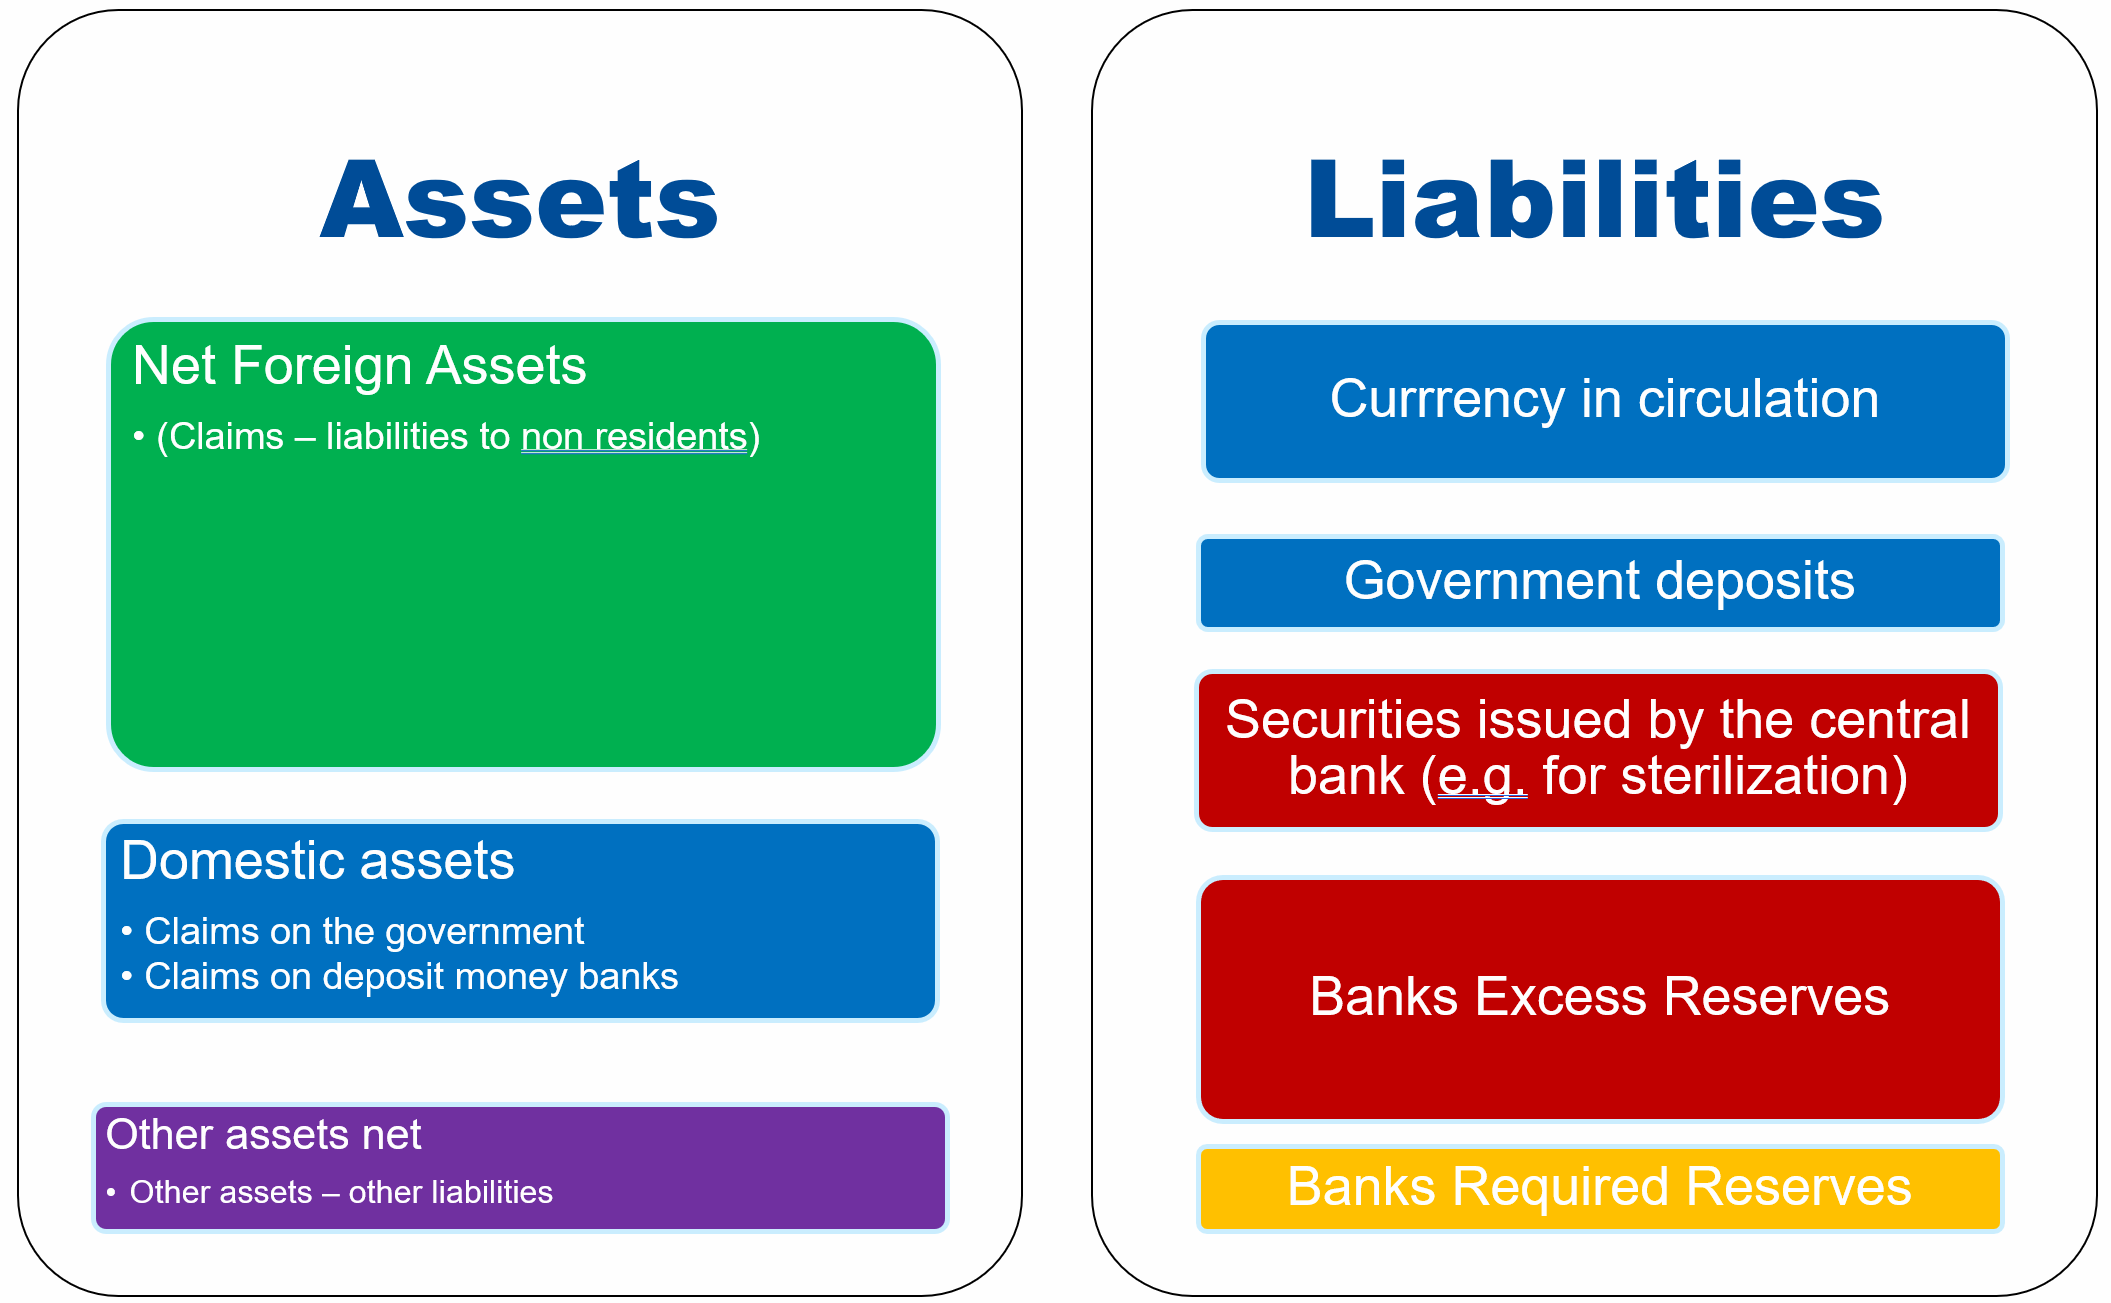
\includegraphics[width=0.75\paperwidth]{img/central_bank_balance_sheet.png}}
\end{frame}


\begin{frame}
  \frametitle{Can All Countries Sterilize?}
  \begin{wideitemize}
  \item In practice, it may be difficult to offset fully the effect of FX interventions
    \begin{itemize}
    \item Countries with under-developed financial markets might not offer enough assets for the central bank to sterilize
    \item Second-round effects of central bank sterilization can dampen
      \begin{itemize}
      \item \emph{For instance: after FXI (buying), sterilization via domestic assets sale, attracts capital inflows, the CB will have to purchase FX further, etc.}
      \end{itemize}
    \end{itemize}
  \item One potential solution: using \textbf{FX derivatives}
    \begin{itemize}
    \item For instance, East-Asian central banks often use FX swaps to sterilize
      \begin{itemize}
      \item Purchasing FX on the spot
      \item Swap by selling FX spot, buying FX in the future
      \end{itemize}
    \end{itemize}
  \end{wideitemize}
\end{frame}


\begin{frame}
  \frametitle{The Costs of Sterilization}
  \begin{wideitemize}
    
  \item \textbf{Fiscal cost}
    \begin{itemize}
    \item Depends on the interest rate differential between domestic and foreign assets
    \item Balance the cost of the conduct of monetary policy with the monetary policy mandate. Important to be consistent, even if it implies costs for the central bank
      \begin{itemize}
      \item Some central banks try to pass the costs to the banking sector, either via the required reserves (FX or domestic, high ratio with below-market remuneration) or forced-holdings of sterilization assets
      \item This is a form of financial repression, and is not advised...
      \end{itemize}
    \end{itemize}
    
  \item \textbf{Valuation risk}
    \begin{itemize}
    \item If foreign reserves grow too much, they expose the central bank to foreign exchange risk
    \item If the foreign currency depreciates, the valuation losses on the FX reserves will reduce the central bank equity
      \begin{itemize}
      \item For instance, the Swiss National Bank (SNB) had to intervene to prevent an appreciation of the Franc that ended up FX reserves representing 130\% of GDP, x12 since 
       \item Valuation losses in 2022 of 95 bn CHF (105 bn USD), or 15 \% of GDP... (were absorbed by SNB very large equity buffer)
      \end{itemize}
    \end{itemize}
    
  \end{wideitemize}
\end{frame}


\begin{frame}
\frametitle{Central Bank Balance Sheet With Rates and Risk}
    \makebox[\linewidth]{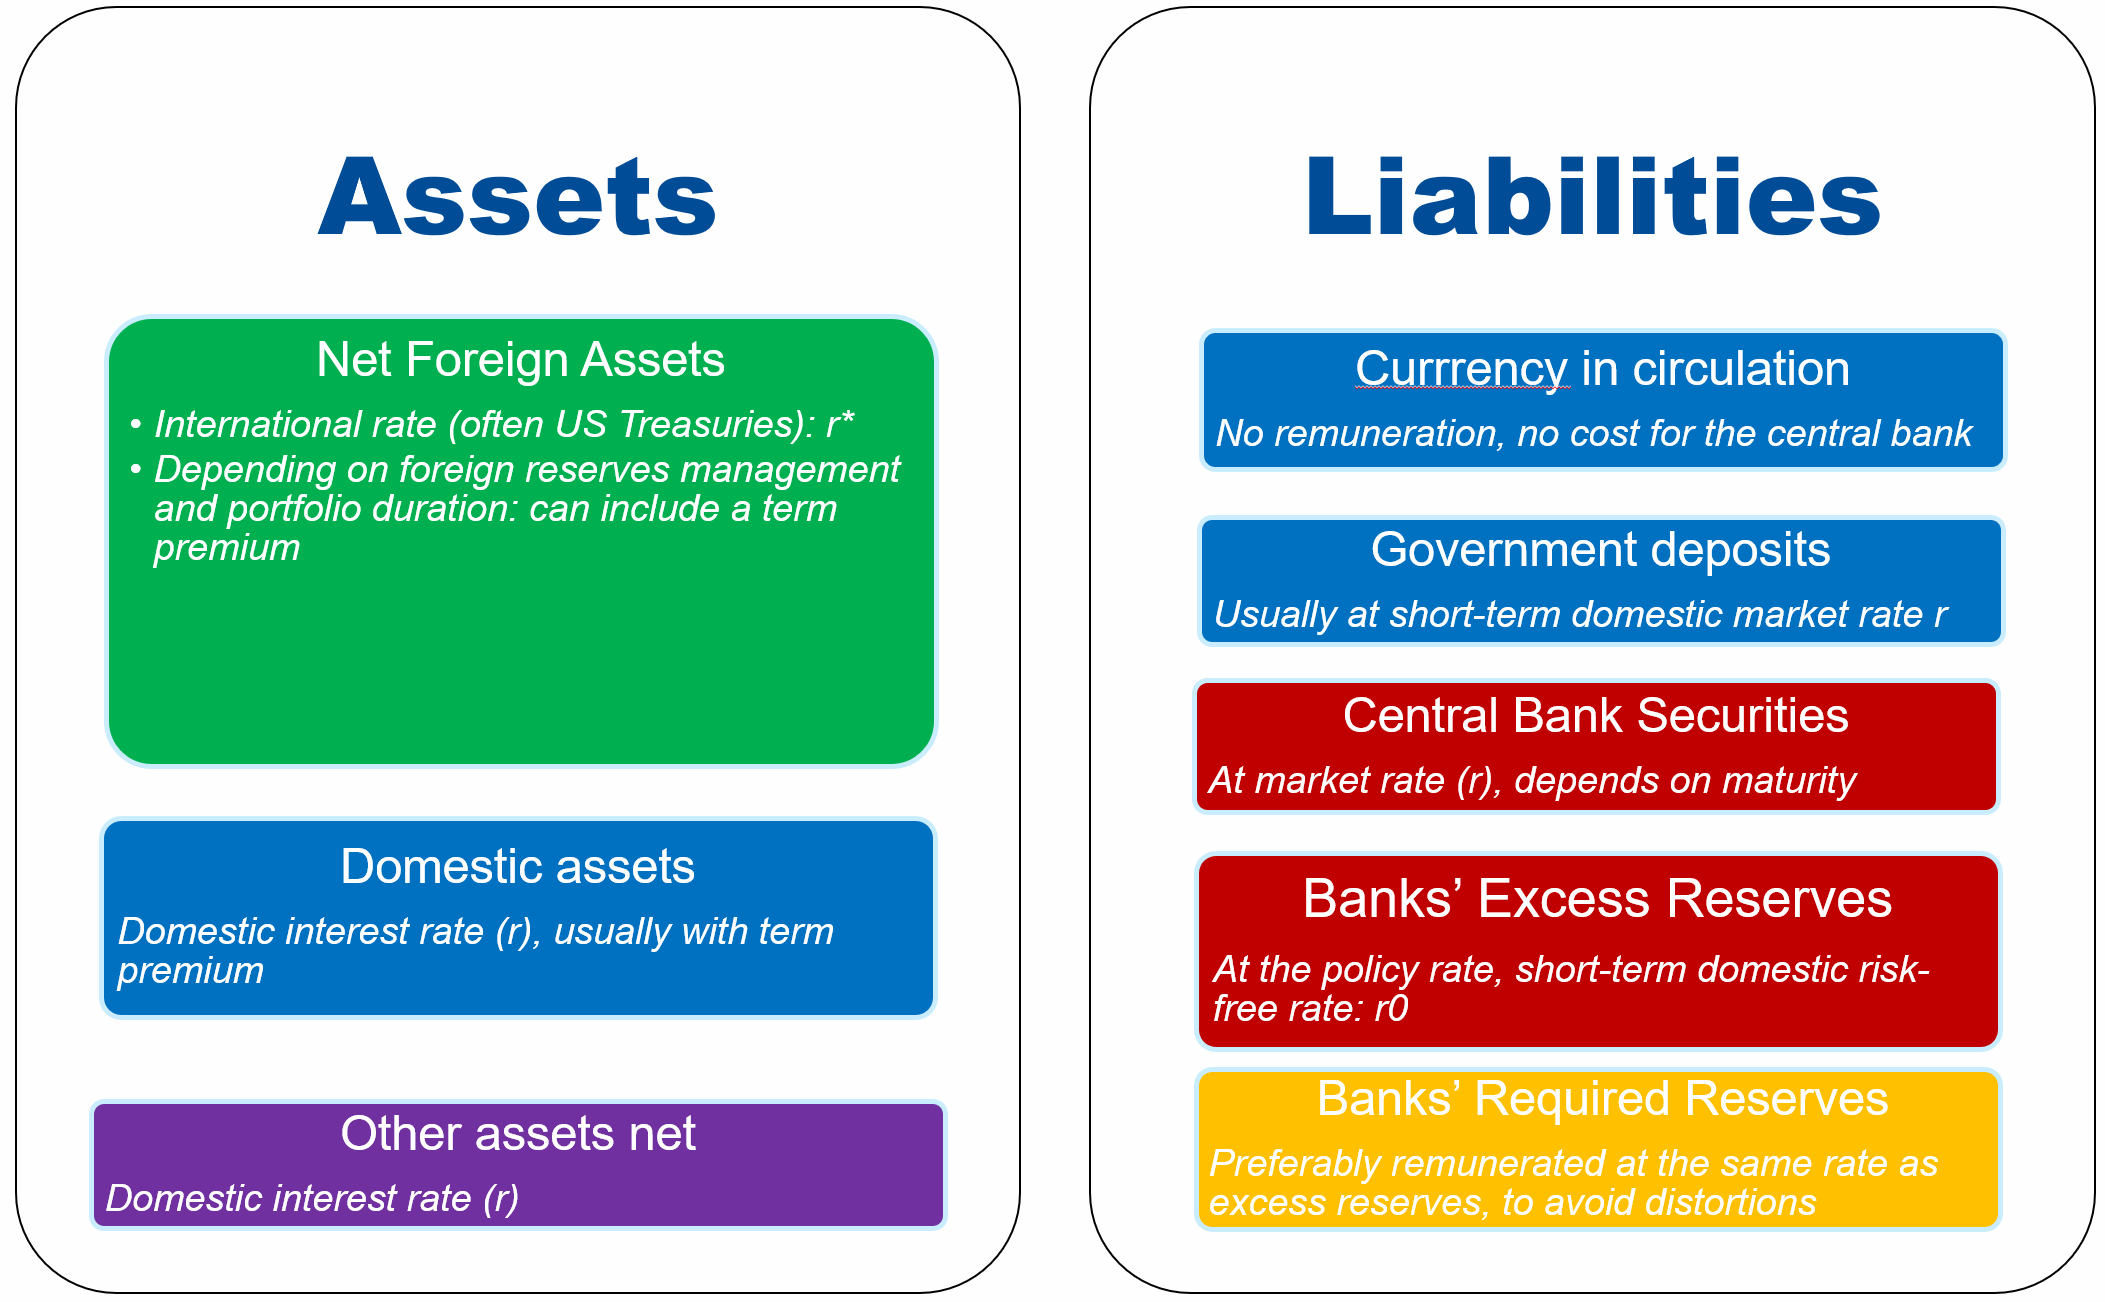
\includegraphics[width=0.75\paperwidth]{img/central_bank_balance_sheet_rates.png}}
\end{frame}


\begin{frame}
\frametitle{PBoC FX Sterilization Costs}
    \makebox[\linewidth]{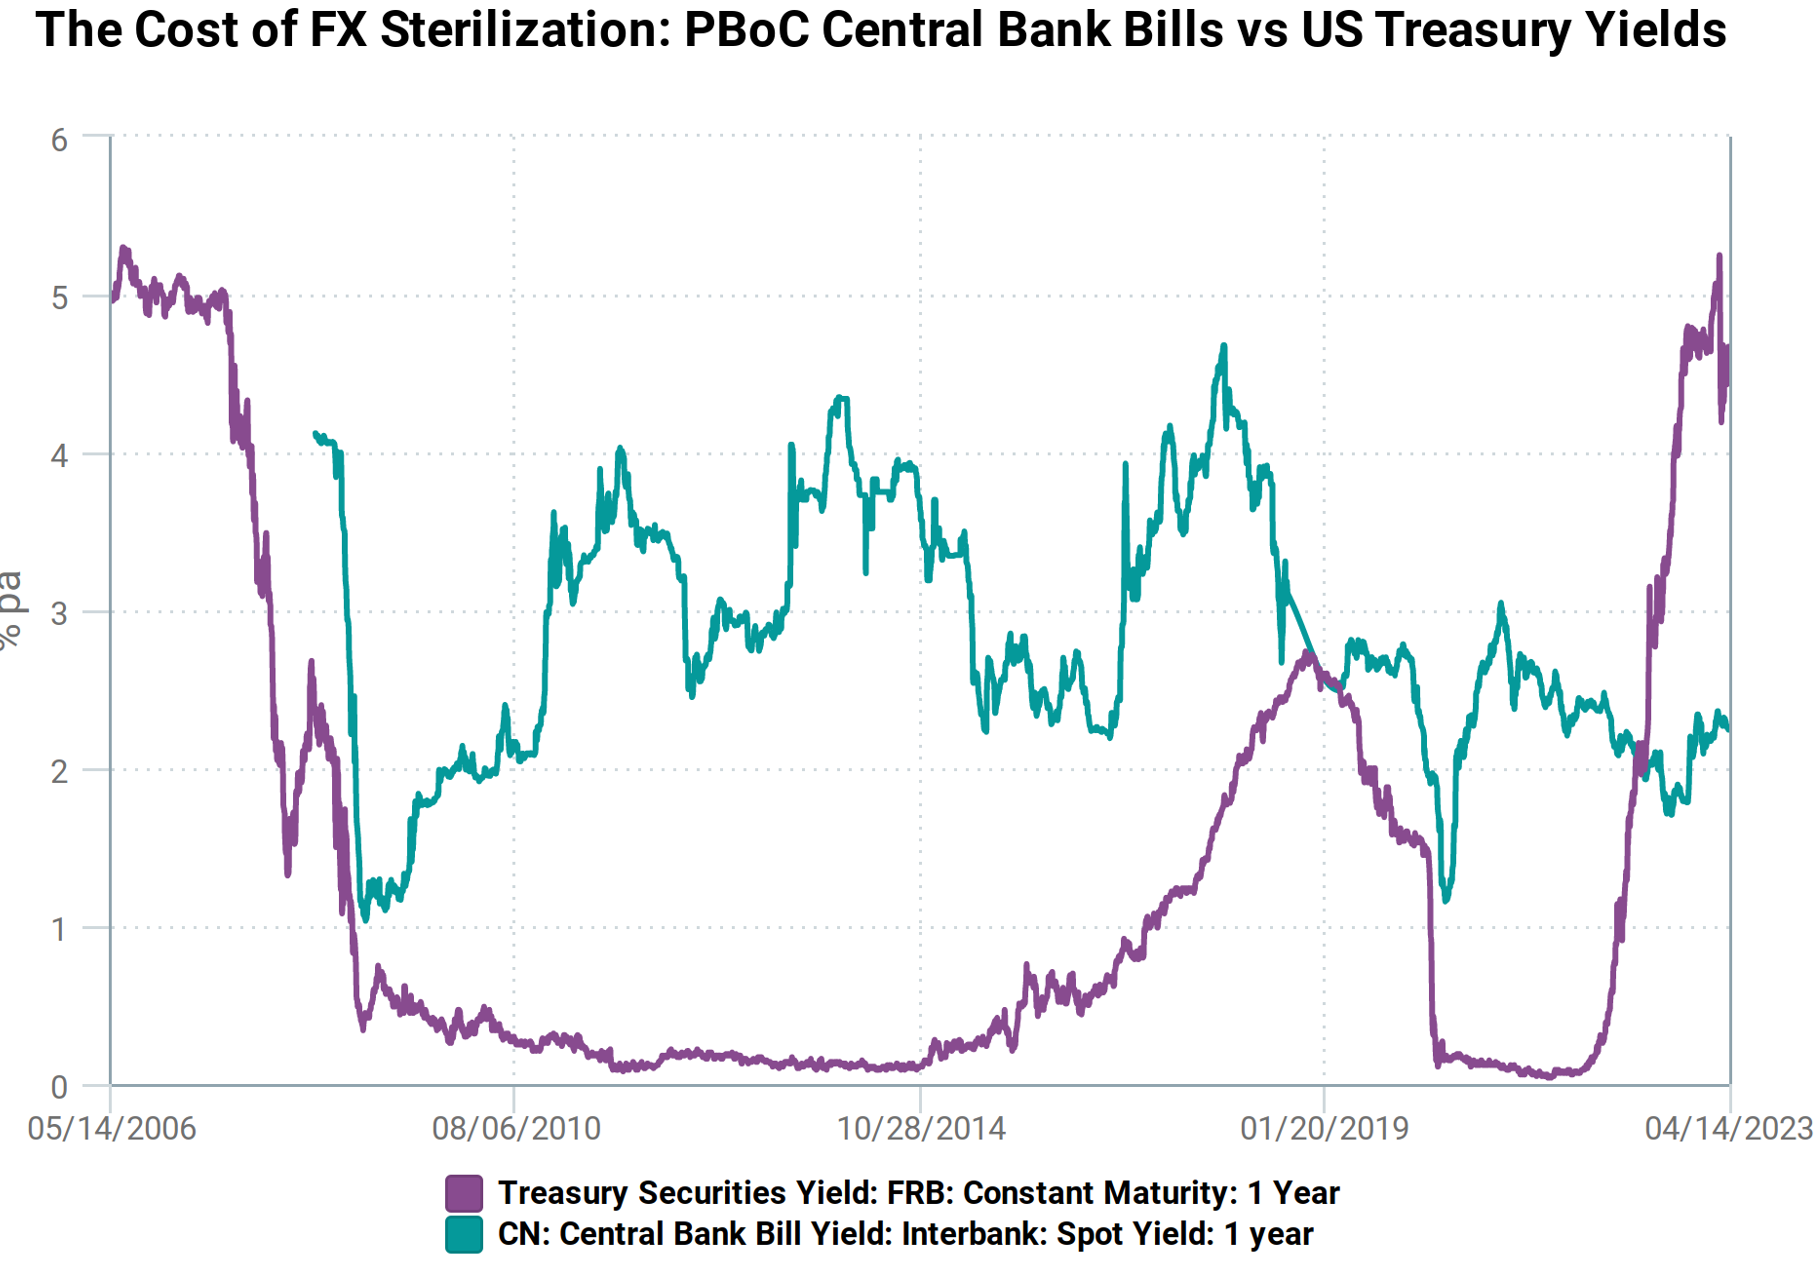
\includegraphics[width=0.75\paperwidth]{img/fx_sterilization_cost_china.PNG}}
\end{frame}


\begin{frame}
\frametitle{PBoC Foreign Reserves}
    \makebox[\linewidth]{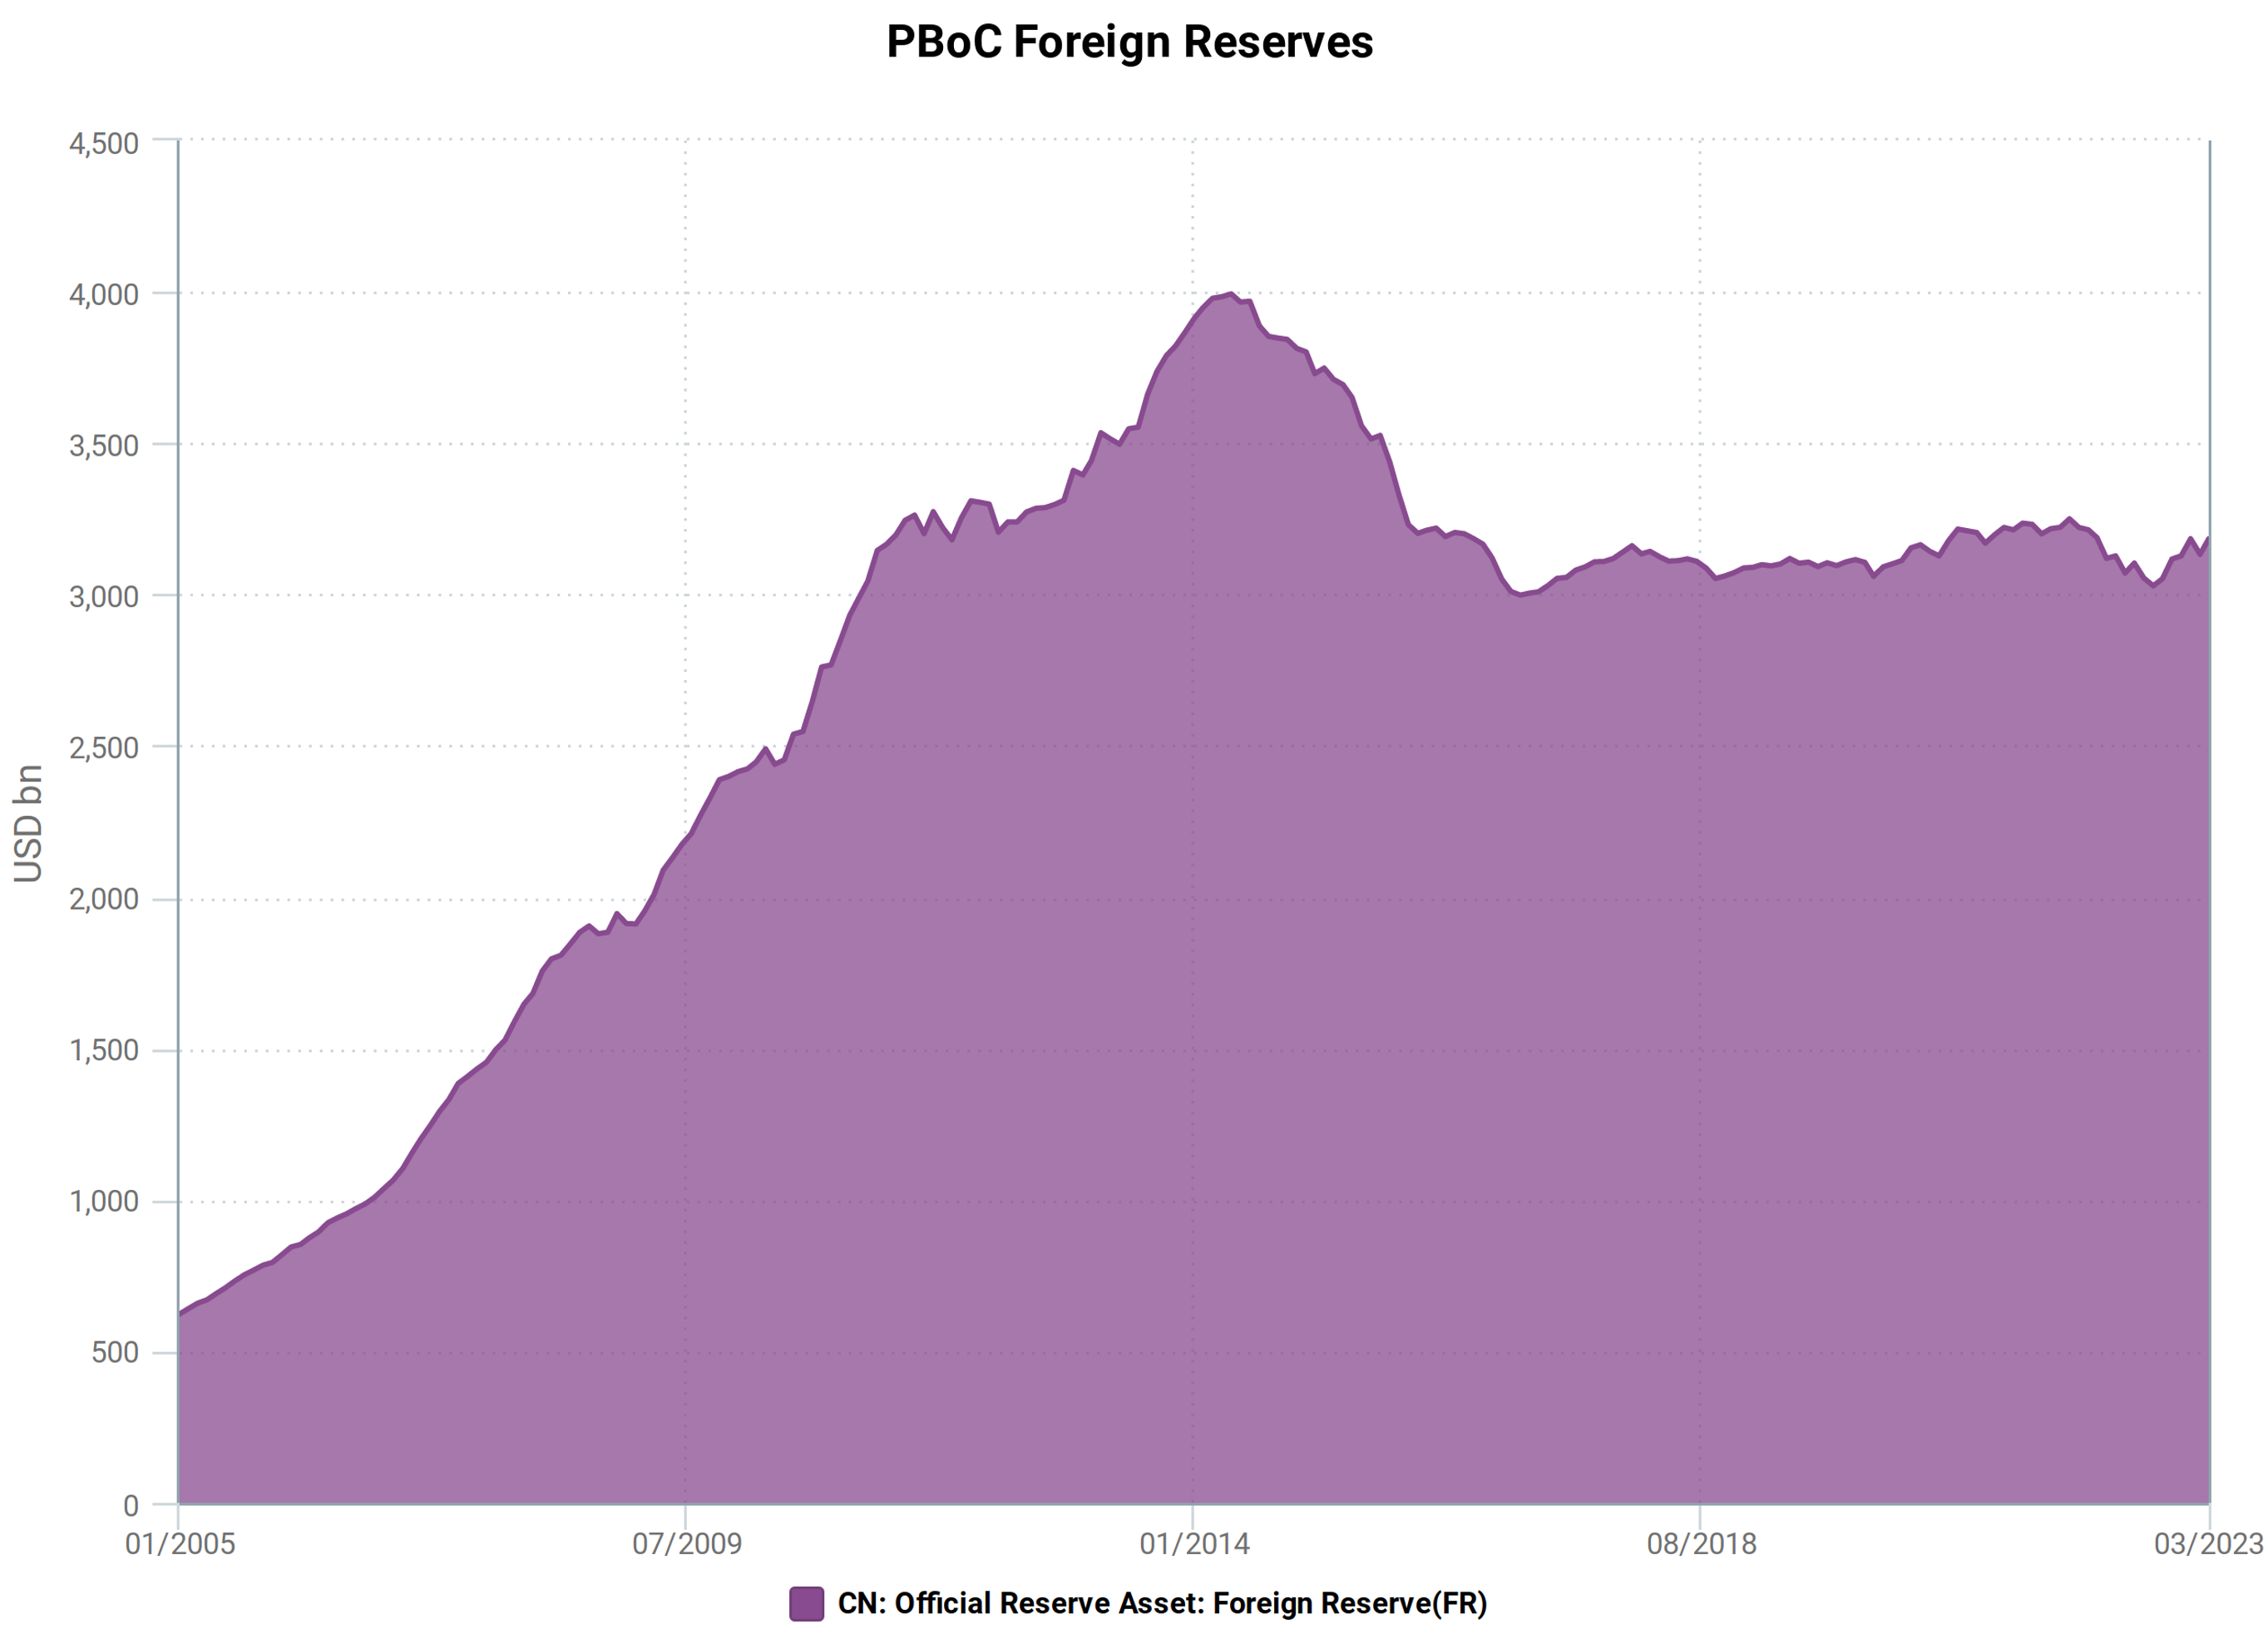
\includegraphics[width=0.75\paperwidth]{img/pboc_fx_reserves.PNG}}
\end{frame}


\begin{frame}
\frametitle{Franc Suisse against Euro (Down Means CHF Appreciation)}
    \makebox[\linewidth]{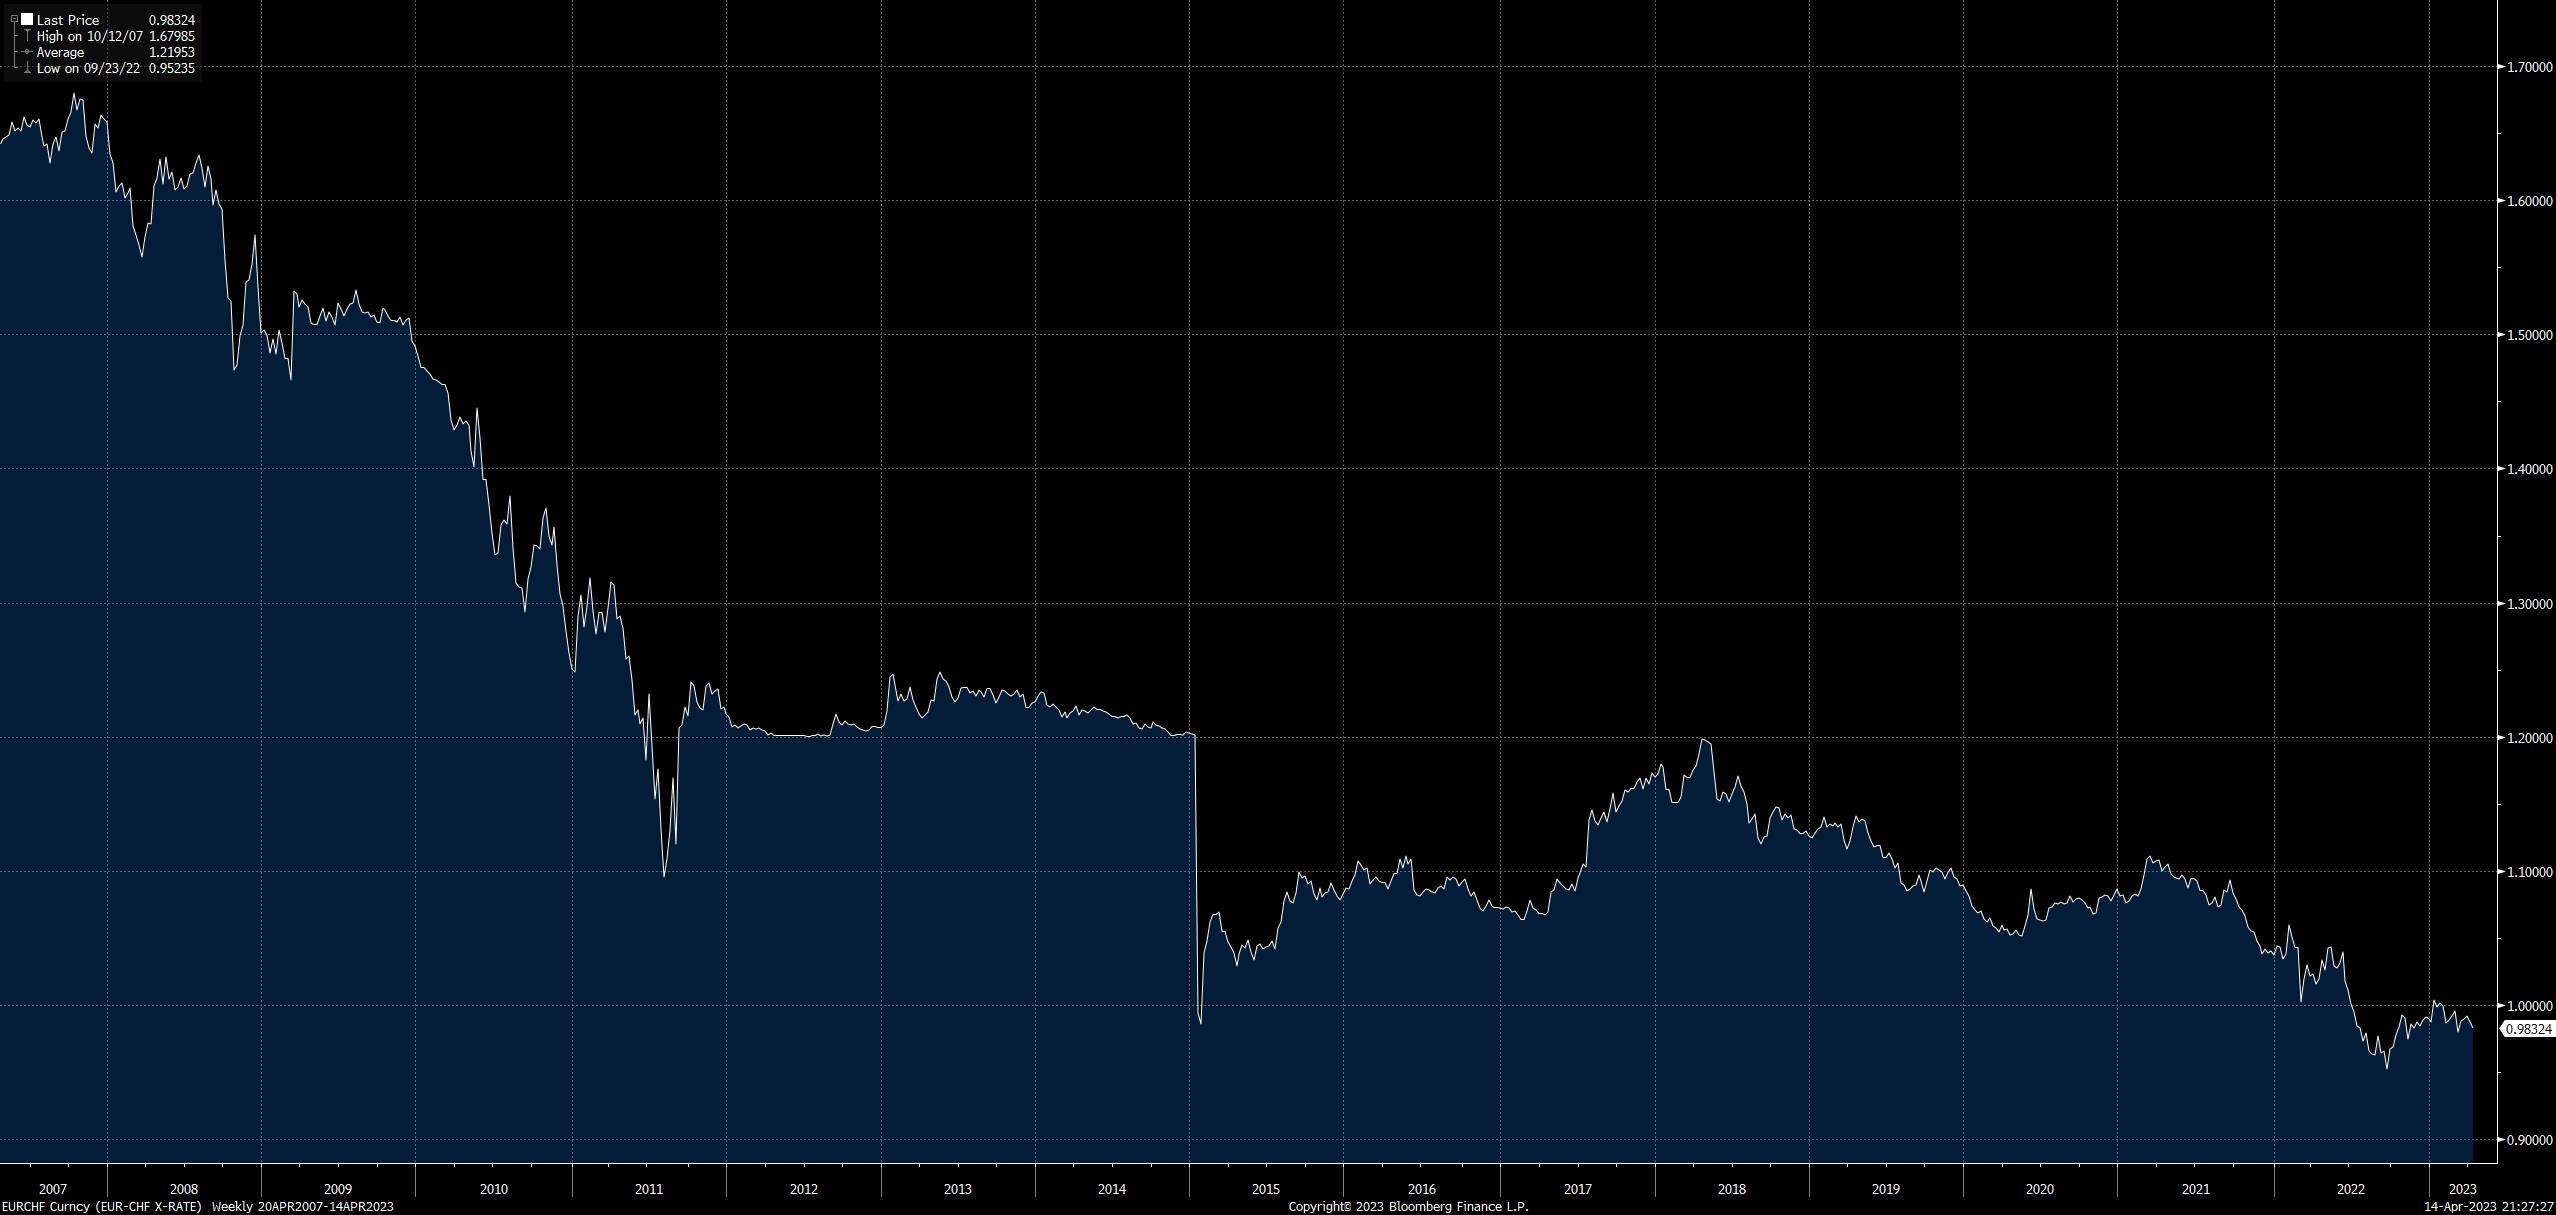
\includegraphics[width=0.75\paperwidth]{img/chfeur.jpg}}
\end{frame}


\begin{frame}
\frametitle{Swiss National Bank Balance Sheet}
    \makebox[\linewidth]{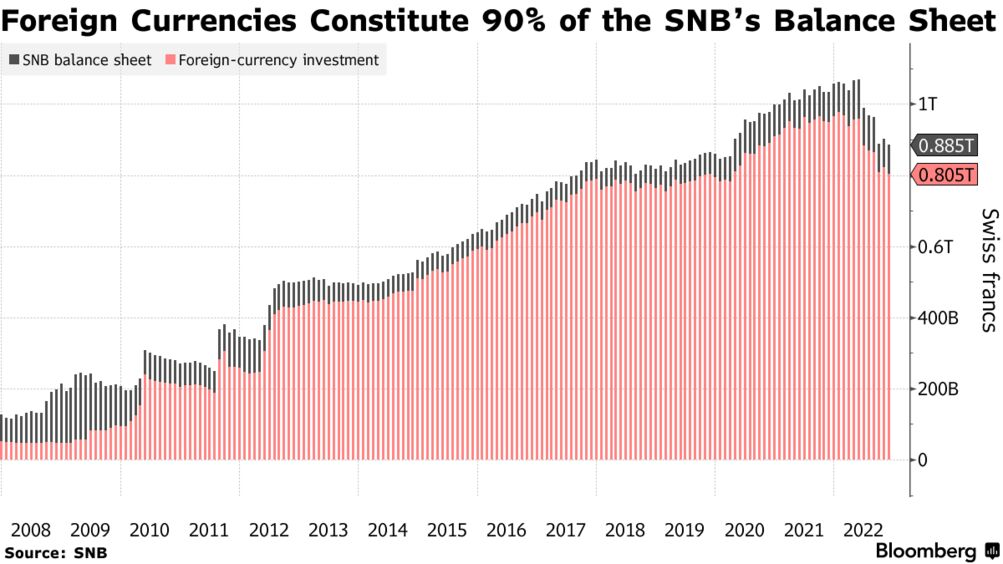
\includegraphics[width=0.75\paperwidth]{img/snb_balance_sheet.png}}
\end{frame}

\begin{frame}
\frametitle{Swiss National Bank Losses}
    \makebox[\linewidth]{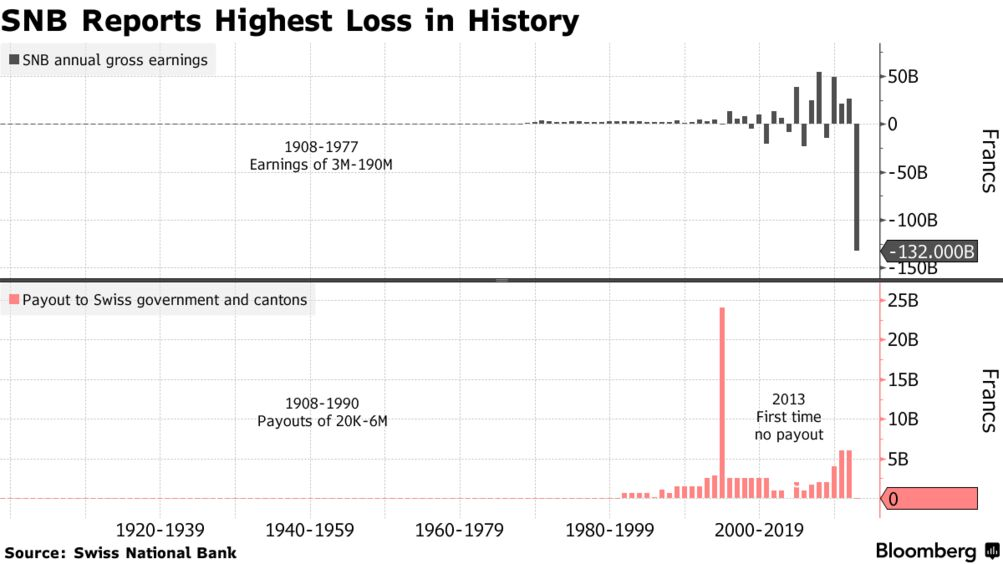
\includegraphics[width=0.75\paperwidth]{img/snb_losses.png}}
\end{frame}


\subsection{Transmission Channels}
\begin{frame}
  \frametitle{Transmission Channels}

  FX interventions influence the exchange rate through two main channels:\\

  \begin{wideenumerate}
  \item Signaling channel
    \begin{itemize}
    \item Signaling future monetary policy stance
    \item Signaling future exchange rate and interventions
    \end{itemize}
  \item Portfolio and risk rebalancing channel    
    \end{wideenumerate}    
\end{frame}


\begin{frame}
  \frametitle{Signaling Channel}
  \begin{wideitemize}
  \item FX Interventions provide investors with "information" about:
    \begin{itemize}
    \item The central bank view of the appropriate exchange rate
    \item The signal of future policy intentions
    \end{itemize}
    
  \item As long as the \textbf{central bank is credible}, the signal can influence the exchange rate
  \end{wideitemize}  
\end{frame}


\begin{frame}
  \frametitle{Signaling and Transparency}
  \begin{wideitemize}
  \item If interventions convey information, why do some central banks continue to keep them secret, even ex-post?
    \begin{itemize}
    \item Threat for the credibility if the intervention is unsuccessful? 
    \item "Wants to keep control", tradition of secrecy
    \item Political repercussions?
    \end{itemize}
    
  \item Rather than conducting FX interventions, why not announcing direct monetary policy changes (e.g. a change in the policy rate)?
    \begin{itemize}
    \item Mussa (1981): "FX interventions may be more credible because it forces the central bank to put money where its mouth is"
    \item In small economies with limited transmission of monetary policy, the exchange rate channel is often the most efficient one
    \end{itemize}
  \end{wideitemize}
\end{frame}


\begin{frame}
  \frametitle{The Portfolio Rebalancing Channel}

  \begin{wideitemize}
  \item Key assumptions of the portfolio rebalancing channel for sterilized FX interventions:\\
    
  \begin{itemize}    
  \item Investors \textbf{diversify their holdings} domestic/foreign as a function of \textbf{expected returns and variance of returns}
  \item \textbf{Foreign and domestic assets are imperfect substitutes}: the uncovered interest parity doesn't hold   
  \end{itemize}

  \item Theory: FXI -> change the relative supply of foreign versus domestic assets -> change expected returns and FX rate
    \begin{itemize}
    \item \emph{For example, after a sterilized FXI selling-side, increase the supply of foreign assets, depreciating the foreign currency}
    \end{itemize}

  \item Sterilized FX interventions also alter the \textbf{risk characteristics} of foreign/domestic assets
    \begin{itemize}
    \item Domestic investors are exposed to FX risk when holding foreign assets
    \item Sterilized interventions influence the equilibrium exchange rate via a change in the \textbf{risk premia}
    \end{itemize}
    
  \end{wideitemize}
\end{frame}


\begin{frame}
  \frametitle{Summary of the Main Transmission Channels}

\begin{tabular}{p{0.2\linewidth}|p{0.3\linewidth}| p{0.3\linewidth}}
\hline
     &  Signaling  &  Portfolio Rebalancing \\ 
\hline
    Assumption &  The central bank is credible &  Assets are imperfect substitutes \\ 
\hline
    Channel & Market Expectations & Relative supply and returns, risk premium \\ 
\hline
\end{tabular}
\end{frame}


\section{Implementation}

\begin{frame}
  \frametitle{Challenges}

  Countries, and in particular EMEs, face implementations issues when framing their FX interventions strategy
  \begin{wideitemize}
    \item Does intervention affect the credibility of inflation-targeting?
    \item Should intervention be discretionary or follow rules?
      \begin{itemize}
      \item If rules, what kind of rules?
      \end{itemize}
  \item What should guide the decision between spot vs derivatives instruments?
  \item Should CBs provide targeted FX provision to specific banks or engage in open-market FX interventions?
  \item Under what conditions is it appropriate to deploy intervention and capital controls jointly?
  \end{wideitemize}
\end{frame}


\begin{frame}
  \frametitle{Different Approaches to Intervention}
  \begin{itemize}
  \item \textbf{Brazil}: discretionary operations, reported one week after since 2008.
    \begin{itemize}
    \item In 2013-2015, daily sales of NDF contracts
    \end{itemize}    
    \item \textbf{Chile}: pre-announced daily purchases of USD 50m with a discretionary intra-day timing
    \item \textbf{Colombia}: 3-minute Dutch auction (descending price) of sales of USD, 20m per day
      \begin{itemize}
      \item discretionary timing: auctions announced in advance, unsold dollars are carried forward the next day
      \end{itemize}      
    \item \textbf{Mexico}: Auctions of USD with a minimum price, 3 times daily at pre-announced times and daily amounts (up to 2016)
      \begin{itemize}
      \item Bids made public at the end of each auction (auctions last 5 minutes)
      \item In 2017, new auctions of NDF that pay in pesos
      \end{itemize}      
    \item \textbf{Peru}: Discretionary operations, announced at start of intervention trades, amounts published daily at market close
  \end{itemize}
\end{frame}

\subsection{Instruments}
\begin{frame}
  \frametitle{Instruments for FX Interventions}
  \begin{wideitemize}
    \item \textbf{FX Spot}
    \item \textbf{FX Forward and FX Non-Deliverable Forward}
    \item \textbf{FX Options} 
    \item \textbf{FX Swaps} 
    \item \textbf{FX Repos}
  \end{wideitemize}
\end{frame}


\begin{frame}
  \frametitle{Spot versus Derivatives?}
  \begin{wideitemize}
  \item Using derivative markets allows the central bank to:
    \begin{itemize}
    \item Provide hedges against FX risk
    \item Influence derivative market liquidity (improve spot/derivative market arbitrage)
    \item May limit the use of FX reserves if the derivatives are settled in local currency (NDF)
    \end{itemize}
  \item Example: the use of non-deliverables FX swaps (NDS) by Brazil:
    \begin{itemize}
    \item Settled in local currency: no impact on foreign reserves
    \item Fills market gap in longer-term derivative instruments (serves as risk management insurance)
    \end{itemize}
  \item Also: Use of forwards, non-deliverables forwards, options, etc.
  \end{wideitemize}
\end{frame}

\begin{frame}
  \frametitle{FX Spot}
  \begin{wideitemize}
  \item Standard transaction on the spot market
  \item Direct impact on the exchange rate, no arbitrage transmission needed  
  \item Provide immediate provision
  \item Limited by the size of the foreign reserves when selling
  \item In some countries, the spot market might be less liquid than the derivative market
  \end{wideitemize}
\end{frame}


\begin{frame}
\frametitle{FX Forwards}
\makebox[\linewidth]{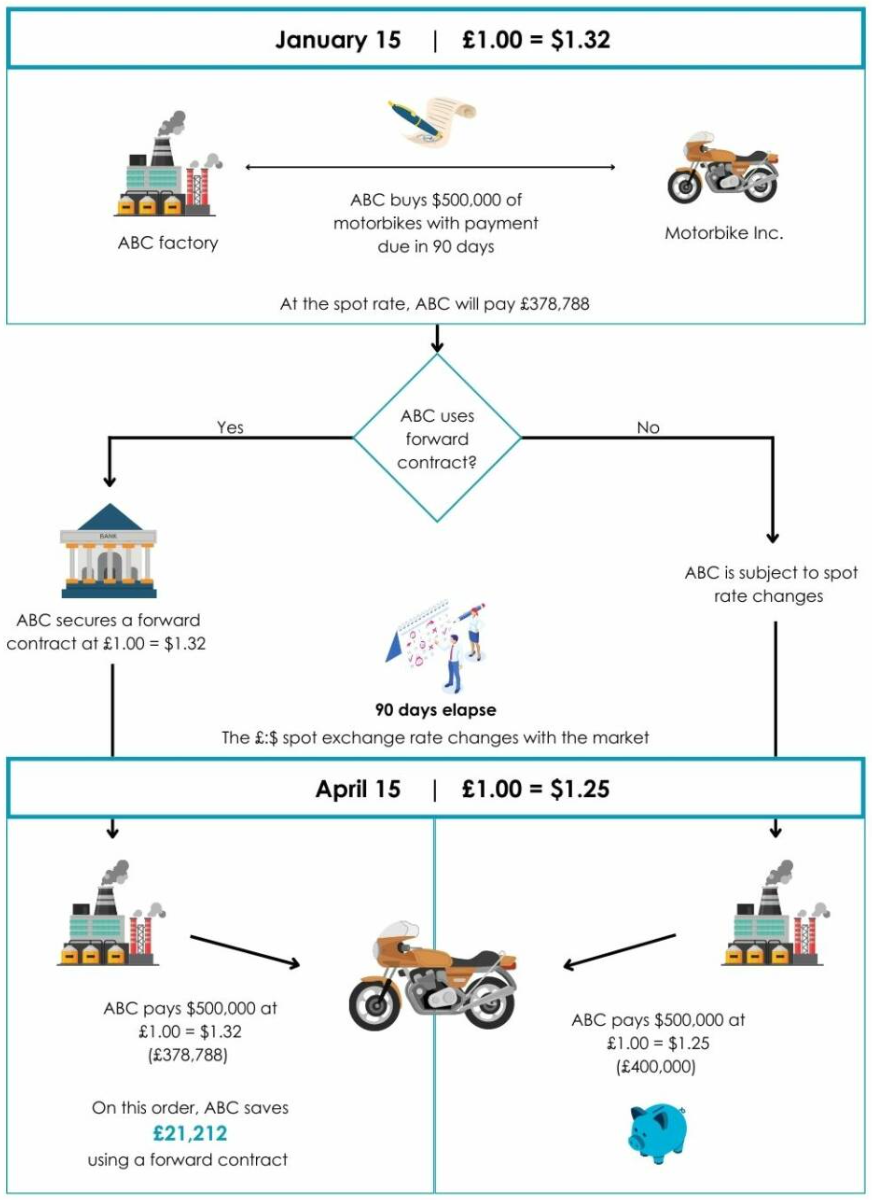
\includegraphics[height=0.75\paperheight]{img/fx_forward_diagram.PNG}}
\medskip
\emph{Source: Trade Finance Global \href{https://www.tradefinanceglobal.com/currency/forward-contracts/)}{\beamergotobutton{Link}}}
\end{frame}


\begin{frame}
  \frametitle{FX Call Options (Protection against Appreciation)}
  \makebox[\linewidth]{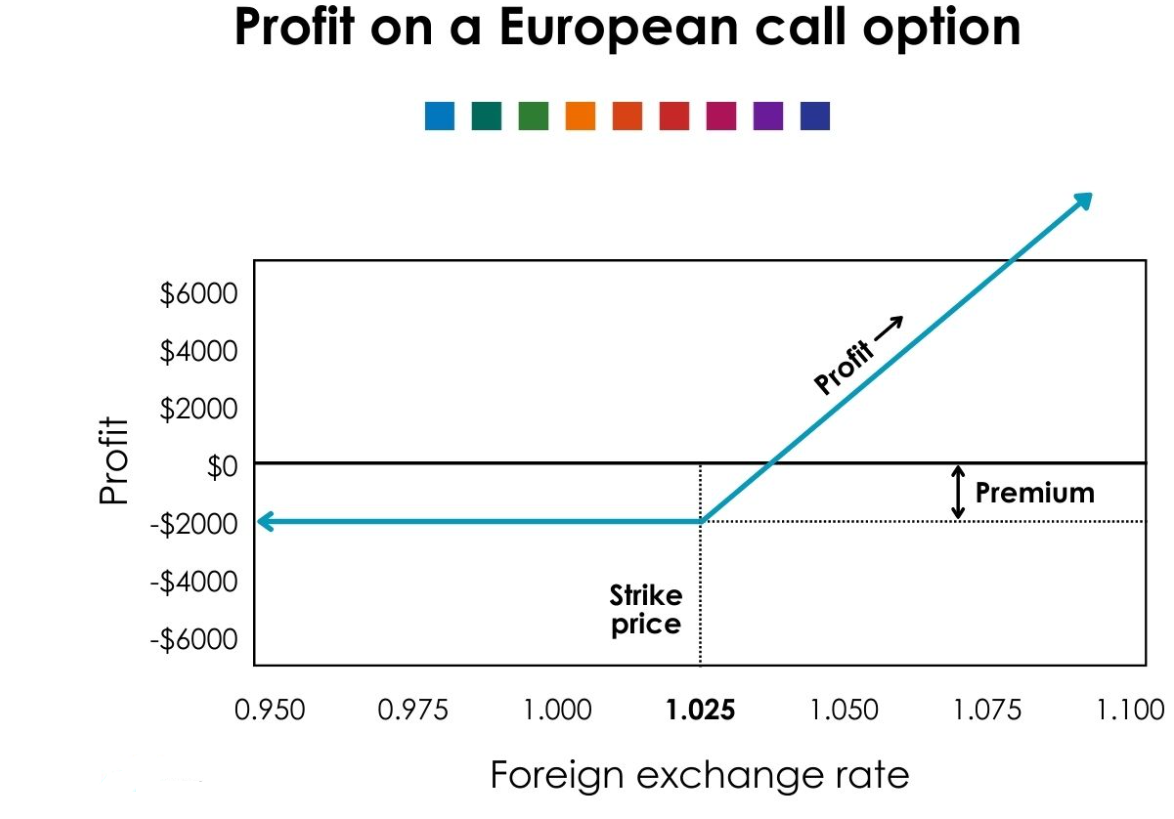
\includegraphics[width=0.75\paperwidth]{img/fx_call_option.PNG}}
  \emph{Source: Trade Finance Global \href{https://www.tradefinanceglobal.com/currency/foreign-exchange-options/)}{\beamergotobutton{Link}}}
\end{frame}


\begin{frame}
  \frametitle{FX Put Options (Protection against Depreciation)}
  \makebox[\linewidth]{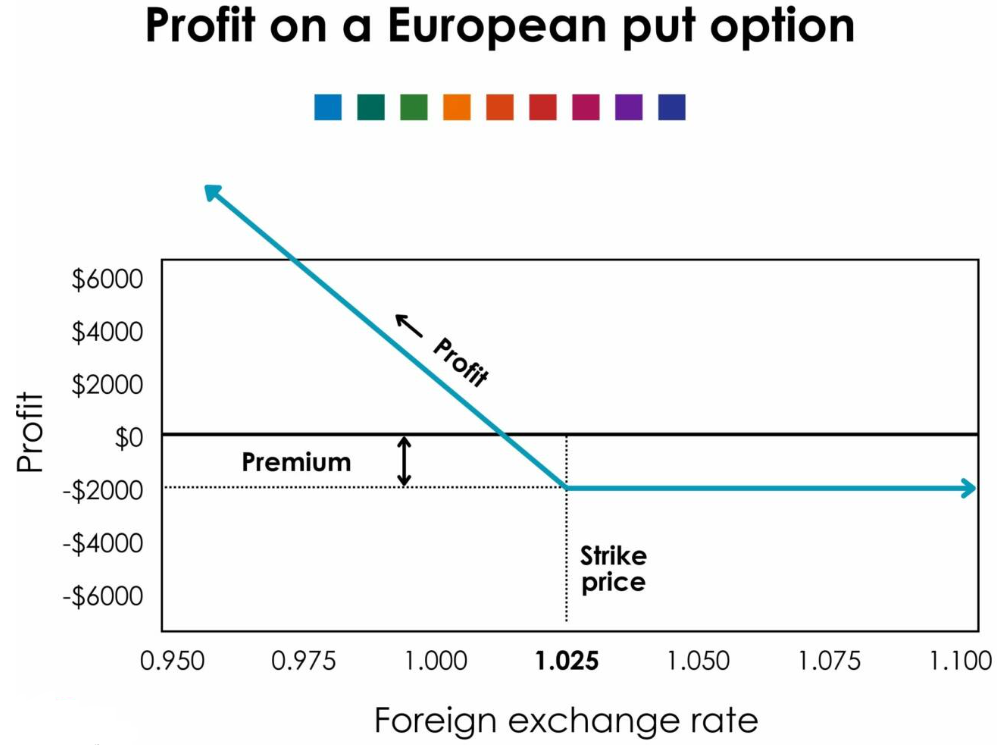
\includegraphics[width=0.75\paperwidth]{img/fx_put_option.PNG}}
  \emph{Source: Trade Finance Global \href{https://www.tradefinanceglobal.com/currency/foreign-exchange-options/)}{\beamergotobutton{Link}}}
\end{frame}


\begin{frame}
\frametitle{Forex Swaps and Cross-Currency Basis Swaps}
\makebox[\linewidth]{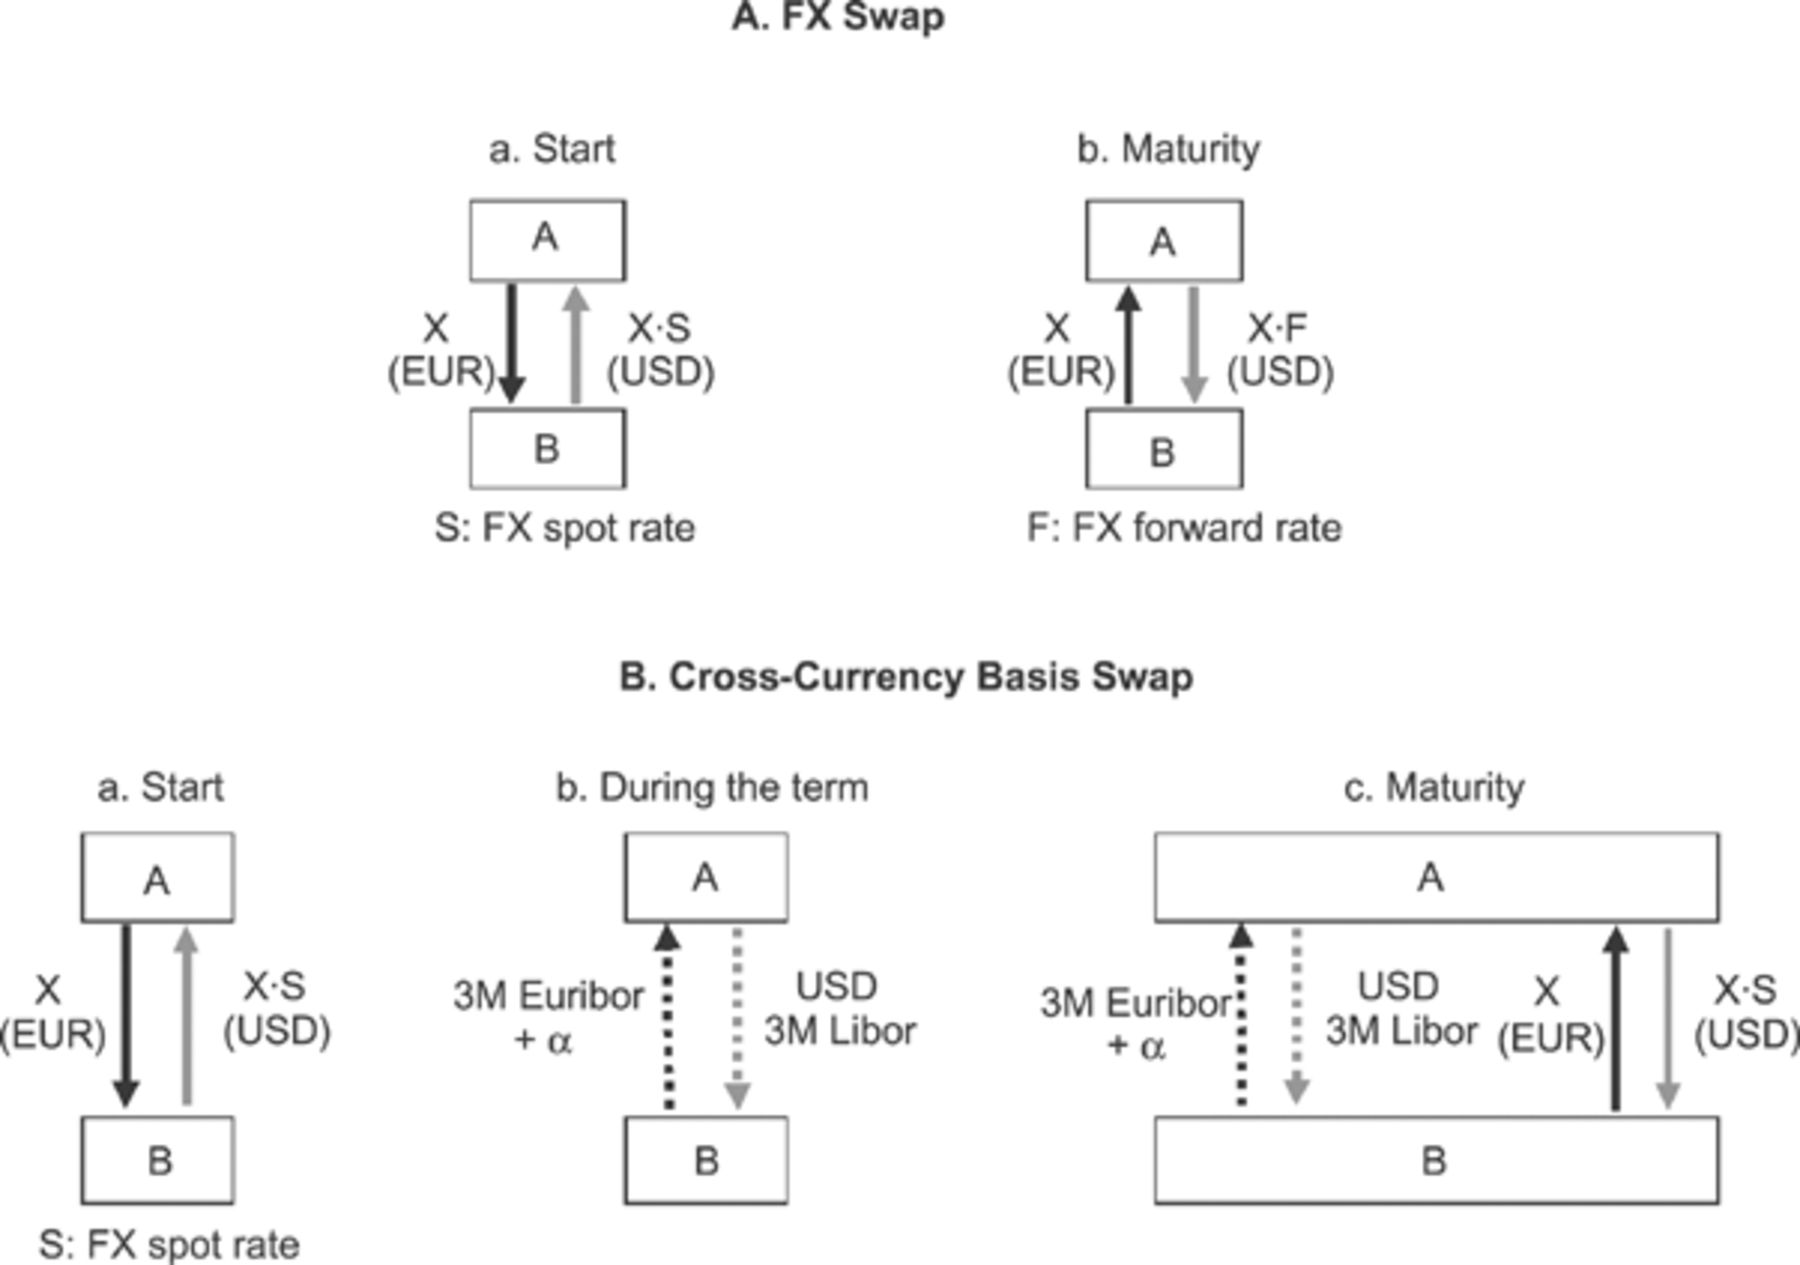
\includegraphics[height=0.5\paperheight]{img/fx_swaps.jpg}}
\medskip
\emph{Source: JFIPM 2008 \href{https://jfi.pm-research.com/content/18/4/24)}{\beamergotobutton{Link}}}
\end{frame}

\begin{frame}
\frametitle{FX Repos and Reverse Repo}
\makebox[\linewidth]{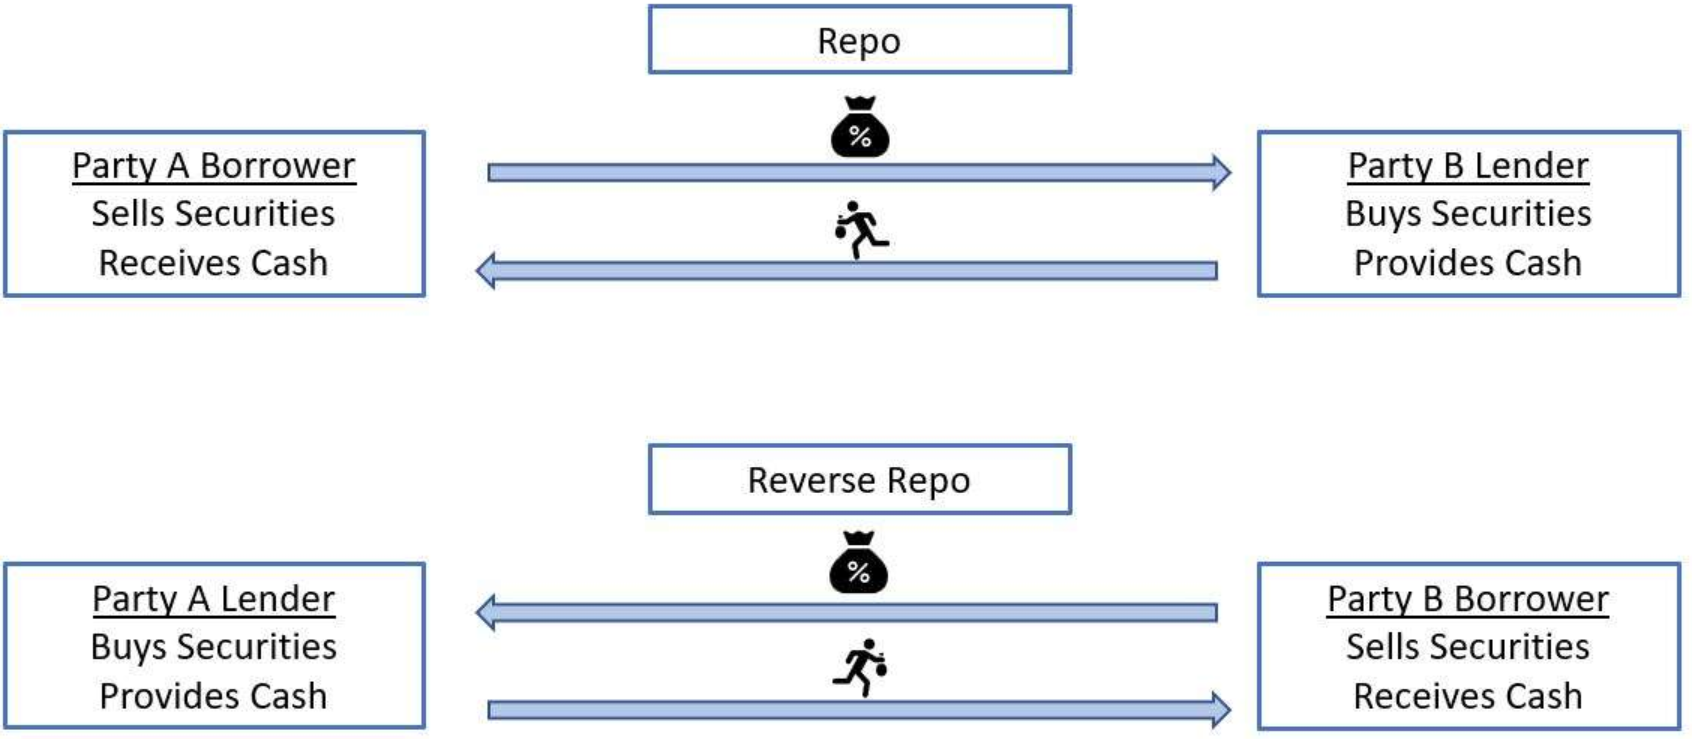
\includegraphics[width=0.75\paperwidth]{img/repo_concept.PNG}}

\bigskip
\emph{Source: Derivativelogic \href{https://derivativelogic.com/wp-content/uploads/Repo-vs-Reverse-Repo.jpg)}{\beamergotobutton{Link}}}
\end{frame}


\begin{frame}
  \frametitle{Spot vs. Derivatives: Intertemporal Considerations}
  \begin{wideitemize}
    \item \textbf{Spot FXI}: provide immediate FX provision
    \item \textbf{Forward FXI}: provide FX at a pre-defined future point in time
    \item \textbf{Option-based FXI}: provide FX during a certain, pre-specified period, in particular turbulent times
    \item \textbf{Repo and swap-based FXI}: provide FX for the duration of the repo or swap, providing a hedge against maturity mismatches in FX
  \end{wideitemize}
\end{frame}


\begin{frame}
  \frametitle{Implementation Differences between AE and EME}
  \begin{wideitemize}
    \item AEs tend to intervene exclusively in the spot market
    \item Many EME countries intervene in derivative markets
      \begin{itemize}
      \item First mover: Bank of Spain sold put options on the peseta to fight devaluation pressures in 1993
      \item Bank of Thailand used forward market purchases to support the baht in 1997
      \item Bank of Mexico sold put options on the USD to accumulate USD reserves in 1990s
      \item Other Latin American countries in the 1990s: Chile, Brazil, Peru
      \item More recently, a growing list of EMEs: Brazil, Colombia, India, Indonesia, Mexico, South-Africa, Thailand
      \end{itemize}
  \end{wideitemize}
\end{frame}

\begin{frame}
\frametitle{Survey of FXI Instruments used by Central Banks}
\makebox[\linewidth]{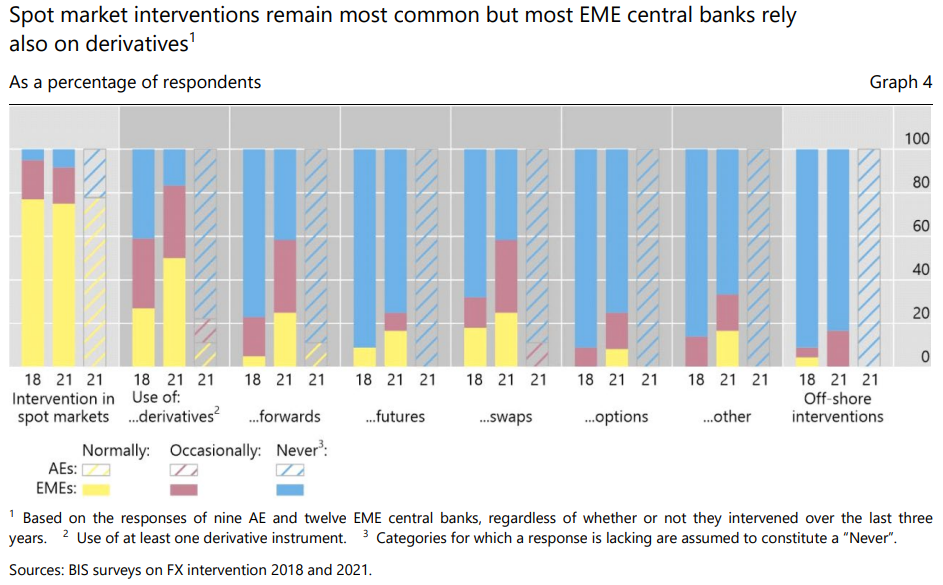
\includegraphics[width=0.75\paperwidth]{img/bis_instruments.PNG}}
\medskip
\emph{Source: BIS 2021 \href{https://www.bis.org/publ/bppdf/bispap104b_rh.pdf)}{\beamergotobutton{Link}}}
\end{frame}


\subsection{Rule vs. Discretion}

\begin{frame}
  \frametitle{Rule vs. Discretion}

  \begin{wideitemize}
  \item Often, central banks prefer to operate via un-disclosed, discretionary interventions
    \begin{itemize}
    \item Idea to "surprise the market"
    \item No commitment of intervention, perceived control on FX reserves level
    \end{itemize}
  \item On the contrary, some central banks use rule-based systems:
    \begin{itemize}
    \item Indicates no explicit intention to target an exchange rate level
    \item Aligned with the monetary objectives
    \item Maximize signaling channel, help agents forming their expectations
    \item Immune to political pressures
    \item Depending on the set-up might give room to speculators
    \end{itemize}
  \end{wideitemize}  
\end{frame}


\begin{frame}
  \frametitle{Rule vs. Discretion}

  \begin{wideitemize}

  \item Countries that have implemented rules-based interventions:
    \begin{itemize}
    \item Mexico, Chile and Columbia: rules-based programs of pre-announced daily purchases/sales of FX
    \item Czech Republic and Russia used to have "automatic interventions"
    \end{itemize}
  \item Evidence from the Czech National Bank \href{https://onlinelibrary.wiley.com/doi/10.1111/jmcb.12028}{\beamergotobutton{Link}} "automated interventions" suggest that rule-based interventions were more effective in steering the FX rate than discretionary interventions
  \item In general, empirical evidence suggest that the effect of discretionary, "surprise" intervention fades very fast    
  \end{wideitemize}  
\end{frame}


\begin{frame}
  \frametitle{BIS Survey on Rule vs Discretion}
  \makebox[\linewidth]{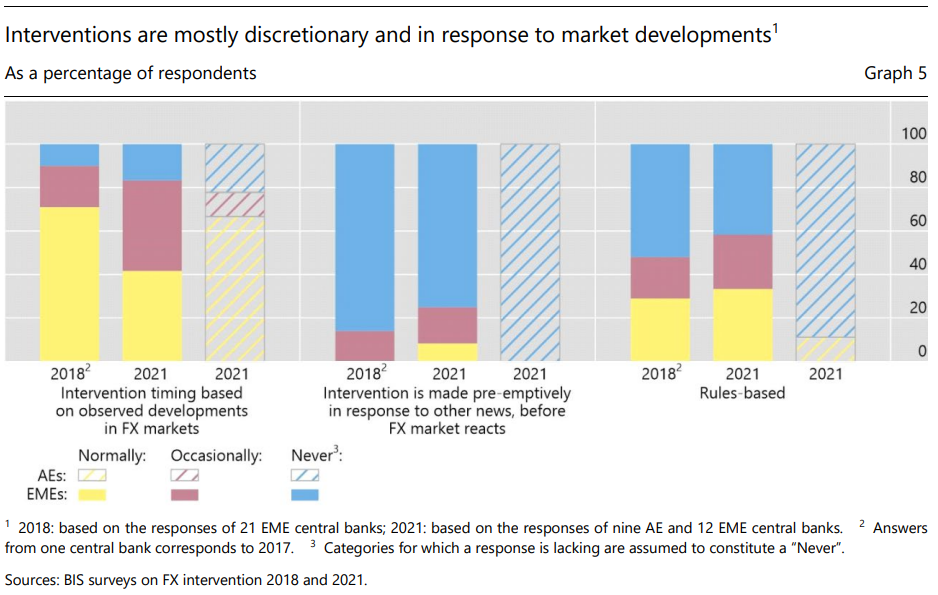
\includegraphics[width=0.75\paperwidth]{img/bis_discretion_rule.PNG}}
  \medskip
  \emph{Source: BIS 2021 \href{https://www.bis.org/publ/mc_insights_fxinterventions.pdf}{\beamergotobutton{Link}}}
\end{frame}

\begin{frame}
  \frametitle{Assessing Central Banks' Rules/Discretion in Practice}
  \begin{wideitemize}
    \item Central banks often don't follow a rigid rule: it is difficult to quantify their objectives and rationales
    \item Policies are often \textbf{episodic}: frequent in some periods and then none in other periods
    \item Operations largely "lean against the wind" to react against deviations from target
  \end{wideitemize}  
\end{frame}

\subsection{FXI Size}

\begin{frame}
  \frametitle{FX Intervention Size}
  \begin{wideitemize}
  \item To the best of my knowledge, there is no theory determining the optimal amount
  \item The general rule is to intervene infrequently, with relatively large amounts (as share of daily market turnover)
    \begin{itemize}
    \item Impact the market
    \item Maximize signaling effect
    \item Gain credibility
    \end{itemize}
  \item Yet, to decide on a specific amount, it is critical to:
    \begin{itemize}
    \item Consider the level of foreign reserves, and the adequate reserves level (e.g. ARA metric or any other metric)
    \item Calibrate as percent of daily FX market turnover
    \item Assess the liquidity conditions and the FX market impact
    \end{itemize}
  \end{wideitemize}
\end{frame}


\begin{frame}
  \frametitle{Orders of Magnitude}
  \begin{wideitemize}
  \item The BIS has conducted a survey of central banks interventions in 2021 (\href{https://www.bis.org/publ/mc_insights_fxinterventions.pdf}{\beamergotobutton{Link}})
  \item On average, cumulated FXI intervention during a day represent between 15\% and 20\% of market turnover, with some central banks exceeding 50\%
    \begin{itemize}
    \item Representing between 0.3\% and 0.8\% of the monthly FX reserves
    \end{itemize}
  \item For regular interveners, frequency of intervention during "normal years" (not COVID) is around 10-15 days per year
    \begin{itemize}
    \item But climbed up to 80 days in 2020 !
    \end{itemize}
  \end{wideitemize}
\end{frame}

\begin{frame}
  \frametitle{BIS Survey on Size and Frequency}
  \makebox[\linewidth]{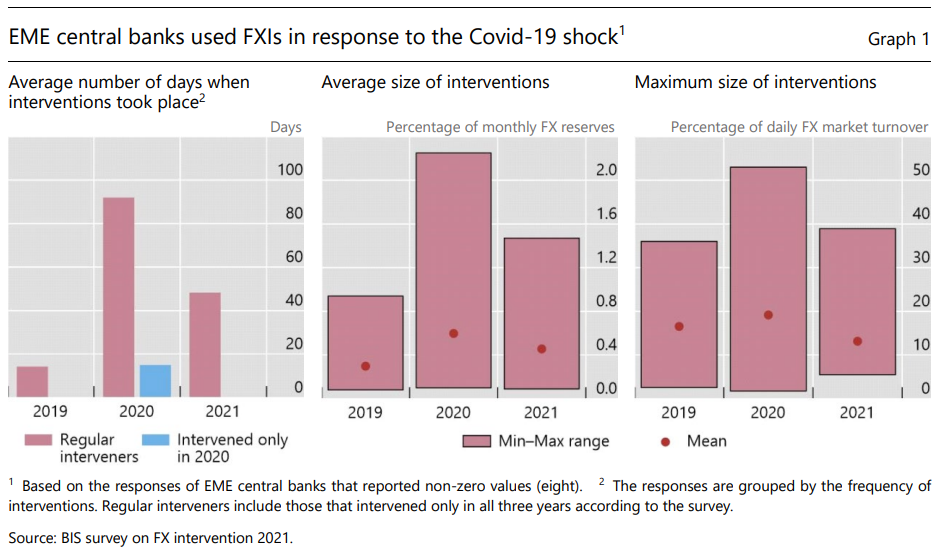
\includegraphics[width=0.75\paperwidth]{img/bis_fxi_size.PNG}}
  \medskip
  \emph{Source: BIS 2021 \href{https://www.bis.org/publ/mc_insights_fxinterventions.pdf}{\beamergotobutton{Link}}}
\end{frame}

\begin{frame}
  \frametitle{Targeted vs. Open Market Interventions}
  \begin{wideitemize}
    \item Systematically important banks may require targeted FX provision under specific circumstances
    \item Even if FX provision facilities are not "targeted", bank take-up is unlikely to be uniform
    \item Issues:
      \begin{itemize}
      \item Potential market distortions and market discriminations among institutions
      \item Political pressures
      \end{itemize}
  \item Open-market more transparent and less distortive
  \end{wideitemize}
\end{frame}


\subsection{Communication}
\begin{frame}
  \frametitle{Communication and Transparency}
  \begin{wideitemize}
  \item Little consensus among central banks, in particular on ex-post communication (data, amounts, etc.)
  \item \textbf{Signaling} is an important transmission channel of foreign exchange interventions and can only be achieved with communication and transparency
  \item The "surprise the market" effect can be detrimental, especially when liquidity is scarce and risk high
    \begin{itemize}
    \item No evidence in the literature that secret and unexpected interventions are more efficient, after the initial first hours
    \item On the contrary, unexpected interventions fade quite fast
    \item Seem to impede anchoring FX market expectations and supporting the credibility of the central bank
    \end{itemize}    
  \end{wideitemize}
\end{frame}



\begin{frame}
  \frametitle{BIS Survey on Ex-Post Communication}
  \makebox[\linewidth]{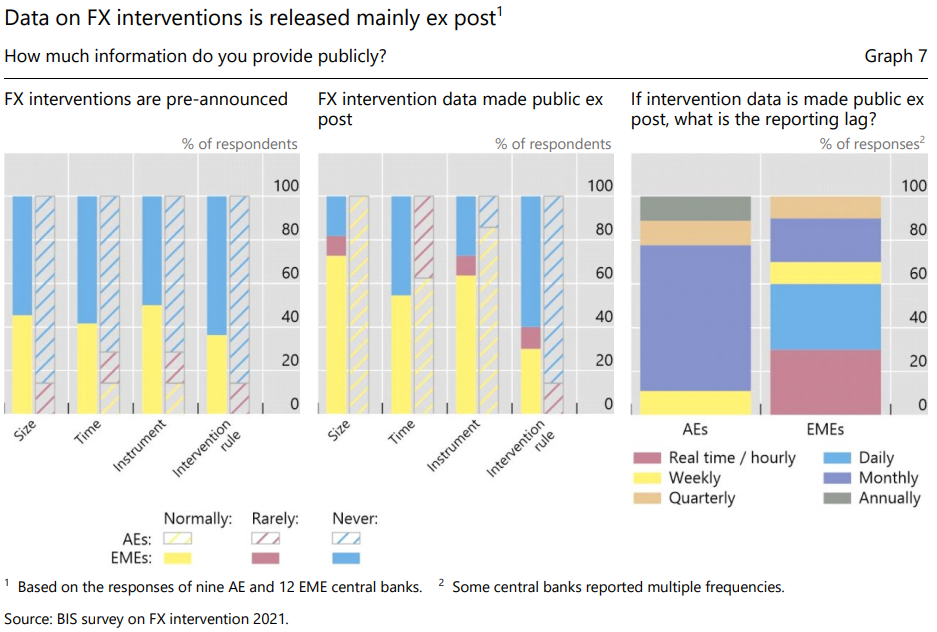
\includegraphics[width=0.75\paperwidth]{img/bis_communication.PNG}}
  \medskip
  \emph{Source: BIS 2021 \href{https://www.bis.org/publ/mc_insights_fxinterventions.pdf}{\beamergotobutton{Link}}}
\end{frame}


\begin{frame}
  \frametitle{BIS Survey on Public Information}
  \makebox[\linewidth]{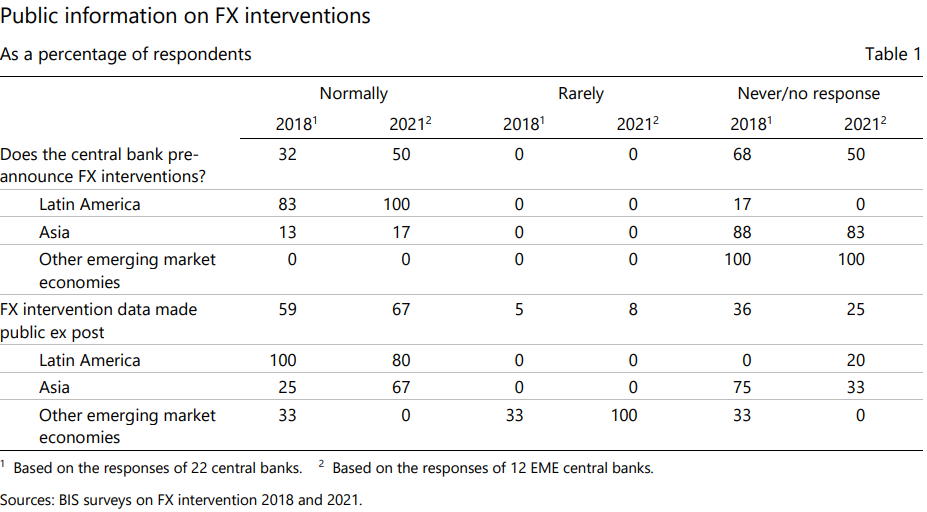
\includegraphics[width=0.75\paperwidth]{img/bis_public_information.PNG}}
  \medskip
  \emph{Source: BIS 2021 \href{https://www.bis.org/publ/mc_insights_fxinterventions.pdf}{\beamergotobutton{Link}}}
\end{frame}


\begin{frame}
  \frametitle{Publicly Available Intervention Data}
  Available via the FRED (Federal Reserve Bank of St Louis):

  \begin{itemize}
  \item Australia (1983-2006)
  \item Germany (1976-1995)
  \item Italy (1988-1998)
  \item Japan (1991-2022)
  \item Mexico (1997-2011)
  \item Switzerland (1975-2001)
  \item Turkey (2002-2019)
  \item United States (1973-2003)
  \end{itemize}

  Central bank websites:
  \begin{itemize}
  \item Argentina
  \item Chile
  \item Georgia
  \item Kyrgyz Republic
  \item United Kingdom
  \end{itemize}  
\end{frame}

\subsection{Intervention Effectiveness}

\begin{frame}
  \frametitle{Technical Issues: Simultaneity}

  \begin{wideitemize}
  \item The decision to intervene is often not independent from movements in exchange rate
    \begin{itemize}
    \item Most likely to occur in reaction to unwanted exchange rate changes
    \end{itemize}
    \item The decision to intervene may also be part of a broader set of policy actions (monetary and/or fiscal policy, capital controls), potentially leading to an \textbf{overestimation bias for intervention}
    \item Studies using high-frequency data (daily, intra-daily) maybe be less subject to the \textbf{simultaneity bias} but can't assess whether intervention has lasting effects
  \end{wideitemize}  
\end{frame}


\begin{frame}
  \frametitle{Criteria for Success}
  \begin{wideitemize}
    \item FXI should significantly influence either the relative price or the volatility of the currency in the appropriate direction
      \begin{itemize}
      \item How large? How persistent? What is the counterfactual
      \end{itemize}
    \item Initial approach: non-parametric test by grouping FXI into "episodes" and test whether the exchange rate movements before/after are consistent with the objectives (Dominguez and Frankel 1993, Fatum and Hutchinson 2003)
      \begin{itemize}
      \item Concern: timing and duration of intervetion episodes are likely to be \textbf{endogeneous}
      \item According to these (old) studies, interventions are generally effective in moving exchange rate in the appropriate direction
      \end{itemize}
  \end{wideitemize}
\end{frame}


\begin{frame}
  \frametitle{Recent Results (Fratzscher 2019, 33 countries 1995-2011)}
  \begin{wideenumerate}
  \item 60\% success in the ability to \textbf{influence the direction of the exchange rate}
    \begin{itemize}
    \item Higher if interventions are large and are accompanied by oral intervention
    \end{itemize}
  \item 80\% success in \textbf{smoothing the path of the exchange rate}
    \begin{itemize}
    \item Reduction in exchange rate variation in the week after the intervention vs the week before
    \end{itemize}
  \item 80\% success to stability the exchange rate in a narrow band
    \begin{itemize}
    \item 2\% band, during the next two weeks
    \end{itemize}
  \end{wideenumerate}
\end{frame}



\begin{frame}
  \frametitle{Interesting Granular Studies}
  \begin{wideitemize}
  \item \textbf{Intraday interventions studies} (BIS 2013) for Chile, Colombia, Mexico, Peru during the GFC
  \item \textbf{Regression discontinuity} (Kuersteiner et al. 2018) on a rule-based intervention Columbia
    \begin{itemize}
    \item Regression: cut-off for triggering the rule is just met or just missed
    \item Idea: variation near the cut-off is almost randomly generated
    \end{itemize}
  \item \textbf{Counterfactual matching approach}: construct a synthetic group as counterfactual
    \begin{itemize}
    \item Not appropriate for frequent intervention but useful at the event level
    \item Counterfactual uses data from other countries, with weights based on the pre-announced co-movement with the currency of interest
    \item Problem in the case of a global shock
    \end{itemize}
    
  \end{wideitemize}
\end{frame}


\begin{frame}
  \frametitle{Profitability of Interventions}
  \begin{wideitemize}
  \item \textbf{Friedman (1953)}: a successful central bank in stabilizing the exchange rate should make a profit at the expense of speculators
    \begin{itemize}
    \item Suggesting that unprofitable interventions are ineffective
    \end{itemize}
  \item \textbf{Edison (1993)}: they show, however, that profitable interventions may have no influence on exchange rates, suggesting flawed Friedman criteria
  \item Empirical evidence suggests that profits vary significantly according to the sample periodm but generally, intervention is profitable
  \end{wideitemize}  
\end{frame}


\subsection{FX Interventions and Exchange Rate Management}

\begin{frame}
  \frametitle{FX Interventions and Capital Flows Management}
  \begin{wideitemize}
    \item Capital flow management (CFM) may increase the efficacy of sterilized FX interventions by reducing foreign and domestic asset substituability
    \item Firms in EME issue more and more foreign currency debt, while EME sovereign debt is increasingly in local currency (with a larger fraction held by foreigners). Therefore:
      \begin{itemize}
      \item Currencies and domestic financing conditions are more exposed to swings in capital flows
      \item EME may need/want full access to all policy tools given these vulnerabilities
      \end{itemize}
    \item Complementary or substitutes?
      \begin{itemize}
      \item FXI is a more flexible tool
      \end{itemize}
  \end{wideitemize}
\end{frame}


\begin{frame}
  \frametitle{Russian Central Bank Intervention}
  \begin{wideitemize}
  \item Unique type of automated intervention
    \begin{itemize}
    \item Place limit orders on an electronic order book to set an upper bound on the rouble price of a dollar
    \item Effectively, Russia was implementing a crawling band to severely limit the flexibility of the rouble
    \end{itemize}
  \item Empirical results \href{https://www.sciencedirect.com/science/article/abs/pii/S0022199609000890}{\beamergotobutton{Link}} at high frequency:
    \begin{itemize}
    \item Russian interventions increased exchange rate volatility for the next few minutes but \textbf{lowered} the degree of volatility over the day, compared to non-intervention days
    \end{itemize}
      \item Case study suggests that countries \textbf{with large reserves and capital controls} can implement a stabilizing crawling exchange rate band using strategic limit orders in electronic currency markets
  \end{wideitemize}
\end{frame}

\begin{frame}
  \frametitle{FX Intervention or Currency Manipulation?}
  \begin{wideitemize}
    \item \textbf{IMF}: The IMF Articles of Agreement prohibit countries from manipulating their currency for the purpose of gaining unfair trade advantage
    \item \textbf{US Treasury approach} (Trade Facilitation and Enforcement Act 2015). Currency manipulation criteria:
      \begin{itemize}
      \item Bilateral trade surplus with the US is at least USD 20 bn
      \item Current account surplus of at least 3 percent of GDP
      \item One-sided intervention (net purchases of foreign currency) conducted repeatedly and totaling at least 2 percent of GDP over a 12-month period
      \item Countries on the "US Monitoring List" if they meet 2 of the 3 criteria: China, Germany, Japan, Korea, Switzerland, India (2018)
      \end{itemize}
  \item In practice, it is very difficult to assert whether a country is manipulating its currency
  \end{wideitemize}  
\end{frame}


\begin{frame}
  \frametitle{When is Exchange Rate Management Warranted?}
  \begin{wideitemize}
    \item Theory: free-floating exchange rate serves as global automatic stabilizers, when markets function efficiently
      \begin{itemize}
      \item Currencies weaken when countries face negative demand or supply shocks, supporting competitiveness
      \end{itemize}
  \item If much of the world experience the negative shock, the stabilization process is less clear-cut
    \begin{itemize}
    \item No impact on exchange rate if all currencies move in the same direction
    \item Currency wars: when many countries try to depreciate their exchange rate
    \end{itemize}
  \end{wideitemize}
\end{frame}


\begin{frame}
  \frametitle{Global Capital Flows Shocks and Exchange Rate Management}

  \begin{wideitemize}
  \item International capital flows can be disconnected with countries' fundamentals and may warrant exchange rate management
  \item Switzerland's experience during the euro crisis is an example of this dilemma
    \begin{itemize}
    \item The Swiss franc appreciated as a safe heaven currency, completely disconnected from Switzerland fundamentals
    \item Massive negative effect on Swiss exporters, and the SNB had to engage into interventions
    \item Establishment of a floor against the Euro (1.20) ... that became unsustainable when the ECB prepared for the QE
    \end{itemize}
  \end{wideitemize}
  
\end{frame}


\begin{frame}
  \frametitle{Can a Country Manipulate its Currency over the Long-Term?}
  \begin{wideitemize}
  \item \textbf{If capital is freely mobile}
    \begin{itemize}
      \item Undervalued exchange rate boost exports -> overheat the economy -> increases domestic prices
      \item Bring the real exchange rate back to an equilibrium value consistent with saving and investment
      \end{itemize}
    \item \textbf{If capital flows are controlled}
      \begin{itemize}
      \item A central bank financing its FX reserves by issuing domestic instruments can force the private sector to increase its net saving
      \item Consequently, the domestic interest rate will rise, and it can deviate from the world interest rate due to capital control
      \item The real exchange rate will deviate from its past equilibrium
      \item Change the balance of saving and investment in the country, potentially weakening its fundamentals
      \end{itemize}
  \end{wideitemize}
\end{frame}


%% ---------------------------------------------------------------------------
%% Case studies
%% ---------------------------------------------------------------------------
\section{Practical Cases}

\subsection{Mexico}

\begin{frame}
  \frametitle{Mexico Path to Free Float Exchange Rate}
  \makebox[\linewidth]{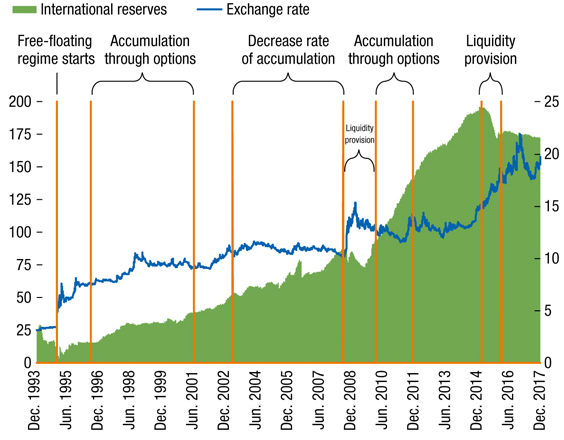
\includegraphics[width=0.5\paperwidth]{img/mexico_timeline.PNG}}
  \medskip
  \emph{Source: IMF \href{https://www.elibrary.imf.org/display/book/9781484375686/ch010.xml}{\beamergotobutton{Link}}}
\end{frame}


\begin{frame}
  \frametitle{FX Interventions to Manage FX Reserves}
  \begin{wideitemize}
  \item USD remittances from the Federal Public Entities
    \begin{itemize}
    \item Especially PEMEX, the national oil company
    \end{itemize}
  \item When the level of foreign reserves is deemed inadequate, the central bank has resorted to rules-based approaches to buy/sell US dollar from the market with preannounced auction mechanisms, where timing and prices were known in advance 
    \begin{itemize}
    \item Buying USD via the \textbf{sale of US dollar put options} to the market via monthly auctions (1996-2001 and 2010-2011) with two requirements
      \begin{itemize}
      \item The option strike price is the \textbf{fix exchange rate determined by the Bank of Mexico on the previous business day}
      \item The option can only be executed only when the peso exchange rate of exercise \textbf{has appreciated with respect to its 20-day moving average} (meaning buying when USD is cheap)
      \end{itemize}
    \item When the level of foreign reserves was deemed too high due to sterilization costs: selling USD via \textbf{spot auctions} half of the amount accumulated during the previous quarter
    \end{itemize}
  \end{wideitemize}
\end{frame}

\begin{frame}
  \frametitle{FX Sterilized Interventions to Smooth Volatility}

  \begin{wideitemize}
  \item Interventions on the spot market via rules-based auctions
    \begin{itemize}
    \item \textbf{US dollar auctions with and without minimum bid price}
      \begin{itemize}
      \item With minimum bid-price, decided on previous business day +2\% (bid are only eligible if they are above this price, yet it is a multiple price auction)
      \item Without minimum bid-price and without triggering rule. The auctions are interactive, the participants know the bids during the auction and could improve their bid.
      \end{itemize}
      
    \item Auctions of USD-denominated credit lines offered to banks, which they could on-lend to corporates (USD 3.2 billion in 2009)
      \begin{itemize}
      \item \emph{The resources came from the swap line with the Fed, not from the BAM reserves themselves}. The BAM still takes only the counterparty risk
      \item Limit moral-hazard via an auction-based pricing mechanism, revealing true banks' risks ("\emph{no free lunch}")
      \end{itemize}
    \end{itemize}
    
  \item Direct USD sales (discretionary) where the tendered amount and triggers are decided by the BAM FX commission
    \begin{itemize}
    \item Including with institutions outside of the country (in 2017) 
    \end{itemize}
  \end{wideitemize}
  
\end{frame}


\begin{frame}
  \frametitle{Other FX Instruments}
  \begin{wideitemize}
  \item \textbf{Foreign Exchange Hedge Auction Program via NDF Auctions Settled in MXN}
    \begin{itemize}
    \item The BAM wants to sell foreign exchange hedges to participants, without endangering its own FX reserves
    \item Market participants bid for the forward exchange rate they need at the maturity of the contract
      \begin{itemize}
      \item At the end of contract: if the spot is higher than the assigned forward price (depreciation), the commercial bank makes a profit settled in pesos
      \item All ND positions are rolled over unitl the BAM decides to stop them
      \item Note that, even though the all transactions are settled in USD, the central bank is short USD. Which is a potential cost (settled in pesos)
      \end{itemize}
    \end{itemize}
  \item \textbf{Flexible credit line with the IMF to supplement current international reserves}
    \begin{itemize}
    \item  Mexico was one of the first three countries to receive an IMF FCL in 2009 when the program was launched
    \item Initially around USD 47 bn, then USD 90 bn in 2016
    \end{itemize}
  \end{wideitemize}
\end{frame}


\begin{frame}
  \frametitle{Mexico Put Options}
  \makebox[\linewidth]{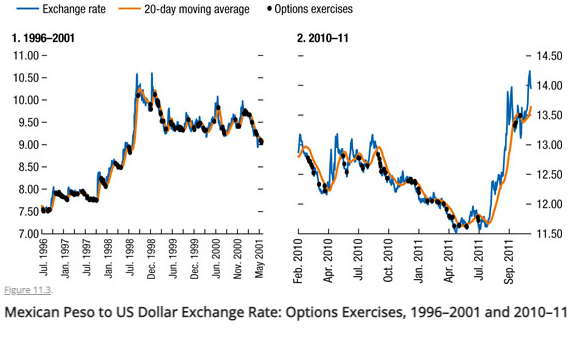
\includegraphics[width=0.5\paperwidth]{img/mexico_put_options.PNG}}
  \medskip
  \emph{Source: IMF \href{https://www.elibrary.imf.org/display/book/9781484375686/ch010.xml}{\beamergotobutton{Link}}}
\end{frame}

\begin{frame}
  \frametitle{Effectiveness}
  \begin{wideitemize}
    \item The BAM interventions framework has been considered by policymakers and the literature as efficient, and without FX target in mind
    \item Empirical evidence suggest that the central bank has been able to contain extreme volatility episodes
    \item Also helping to maintain the policy objective, which is to keep the interbank funding rate at the monetary policy objective

  \end{wideitemize}
\end{frame}

\begin{frame}
  \frametitle{Mexico Interbank Rate}
  \makebox[\linewidth]{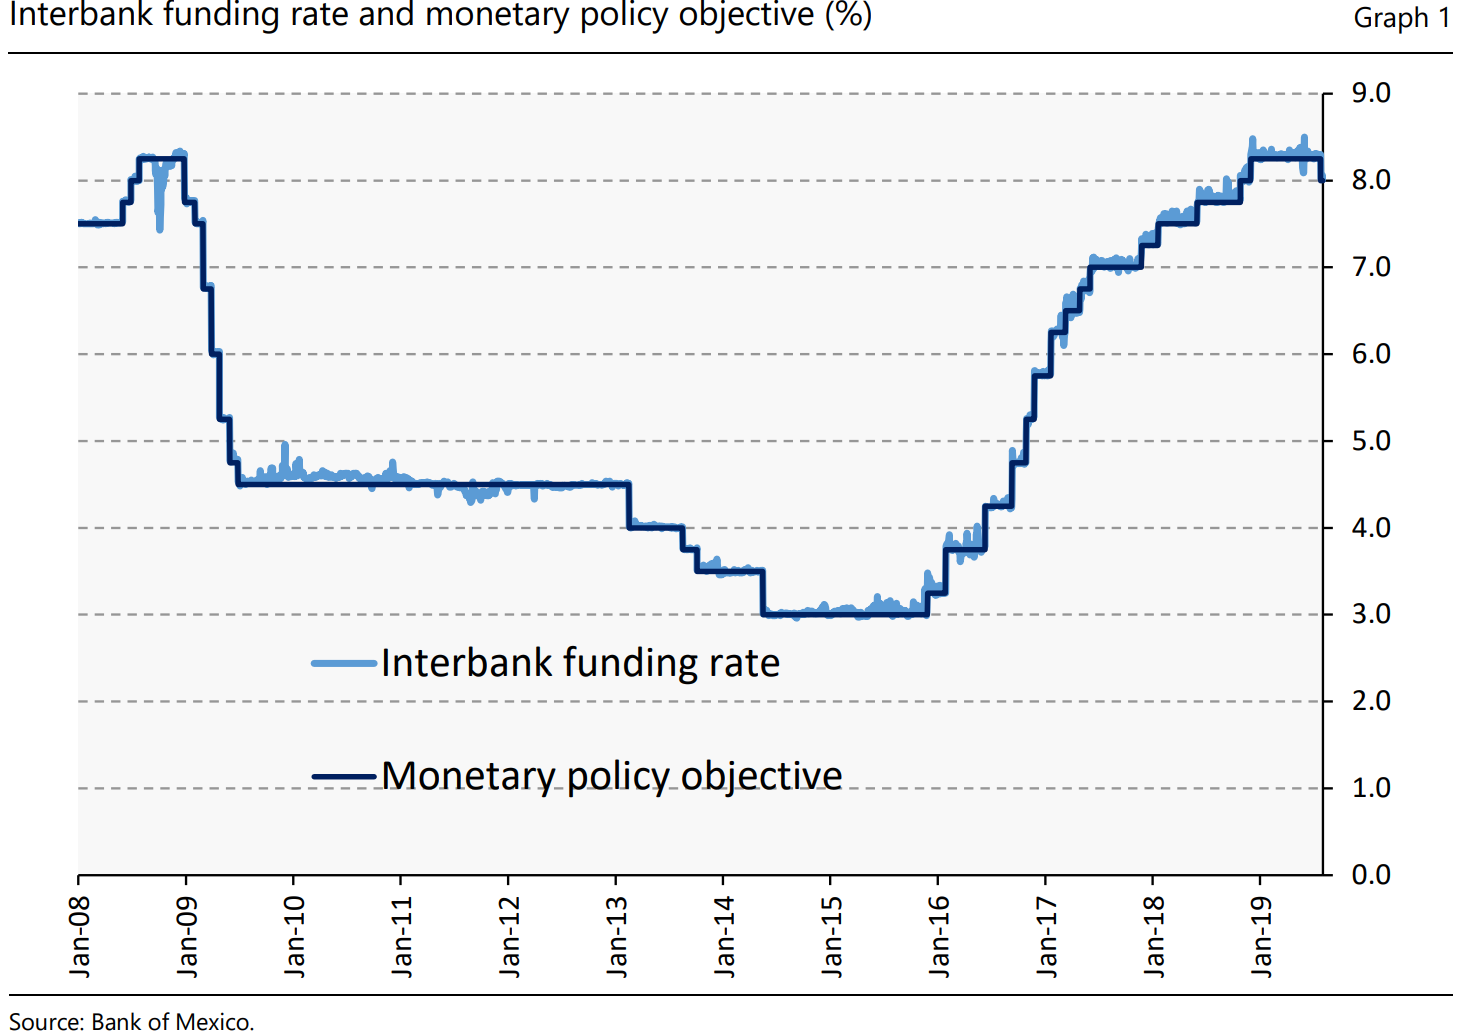
\includegraphics[width=0.75\paperwidth]{img/mexico_interbank_rate.PNG}}
  \medskip
  \emph{Source: Bank of Mexico and BIS \href{https://www.bis.org/publ/bppdf/bispap104p.pdf}{\beamergotobutton{Link}}}

\end{frame}



\subsection{Brazil}

\begin{frame}
  \frametitle{Brazil: During GFC}
  \begin{wideitemize}
  \item During the GFC, the Brazilian central bank used a combination of different instruments to stabilize the BRL
    \begin{itemize}
    \item Swaps
    \item Spot market auctions
    \item Repo market auctions
    \item Trade finance loans
    \item Forward market auctions
    \end{itemize}
  \item Kohlscheen and Andrade (JIMF 2014) find that the currency swaps carried in 2011 Q2-2012 had a significant effect on the BRL/USD
  \end{wideitemize}
\end{frame}

\begin{frame}
  \frametitle{Brazil (2013-2018)}
  \begin{wideitemize}
    \item The BCB implemented the largest ever intervention in the FX derivatives market in August 2013
      \begin{itemize}
      \item Initially to counter-act capital outflows and the BRL depreciation during the "Taper Tantrum"
      \end{itemize}
  \item The open position of the BCB in these derivatives summed up to \textbf{7\% of the Brazilian GDP} (\textbf{30\% of the international reserves}) in the peak of the program in 2015
  \item The intervention program was considered successful and other EME have followed: Mexico (February 2017), Turkey (November 2017)
  \end{wideitemize}
\end{frame}


\begin{frame}
  \frametitle{Brazil 2013: Hedger-of-Last-Resort}
  \begin{wideitemize}
  \item Due to historical restrictions to buy US dollars in the Brazilian sport market, the country's FX derivative markets became larger than the spot one. 
  \item Intervention program: daily sales of USD 500 million worth of currency non-deliverables forwards
    \begin{itemize}
    \item USD forwards settled in BRL, also known as BCB swaps, developped by the BCB (the "swaps cambiais")
    \item Traded in the local stock exchange ("B3")
    \end{itemize}
    
  \end{wideitemize}
\end{frame}

\begin{frame}
  \frametitle{FX Derivatives Players and their Net Exposures}
  \makebox[\linewidth]{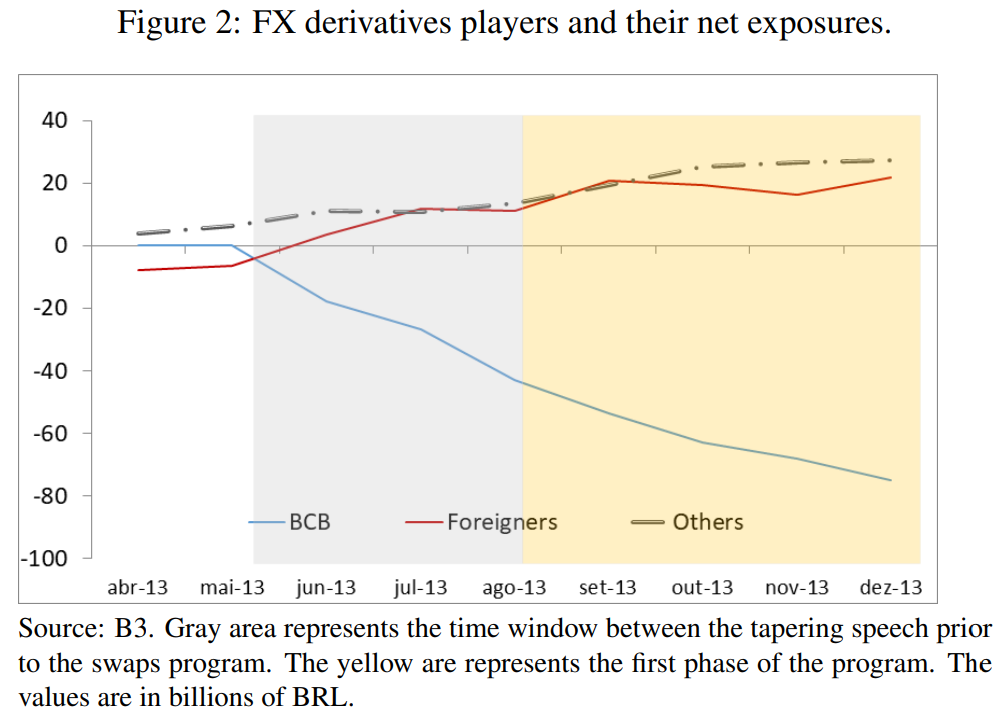
\includegraphics[width=0.75\paperwidth]{img/brazil_hedge_positions.PNG}}
  \medskip
  \emph{Source: Gonzalez, Khametshin, Peydro and Polo (2019)}
\end{frame}


\begin{frame}
  \frametitle{Effects of the August 22 2013 Intervention in the BRL/USD exchange rate}
  \makebox[\linewidth]{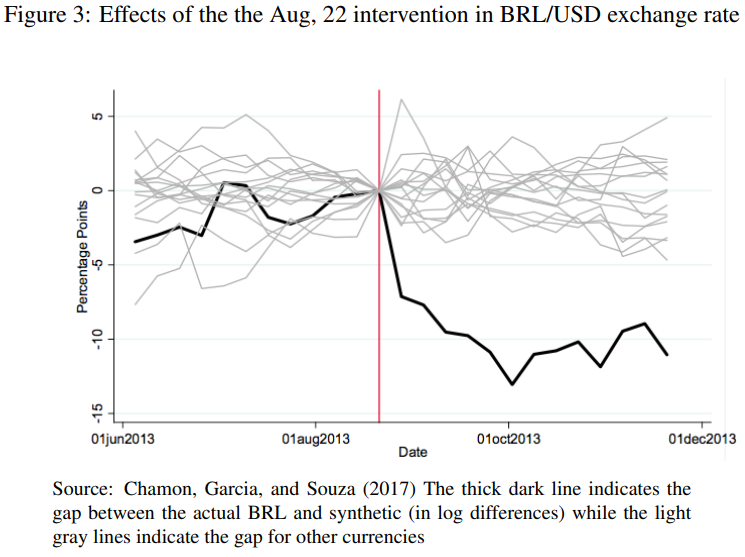
\includegraphics[width=0.75\paperwidth]{img/brazil_intervention_effect.PNG}}
  \medskip
  \emph{Source: Gonzalez, Khametshin, Peydro and Polo (2019)}

\end{frame}


\begin{frame}
  \frametitle{Yet the Effect has been Fading Out between 2013 and 2015}
  \makebox[\linewidth]{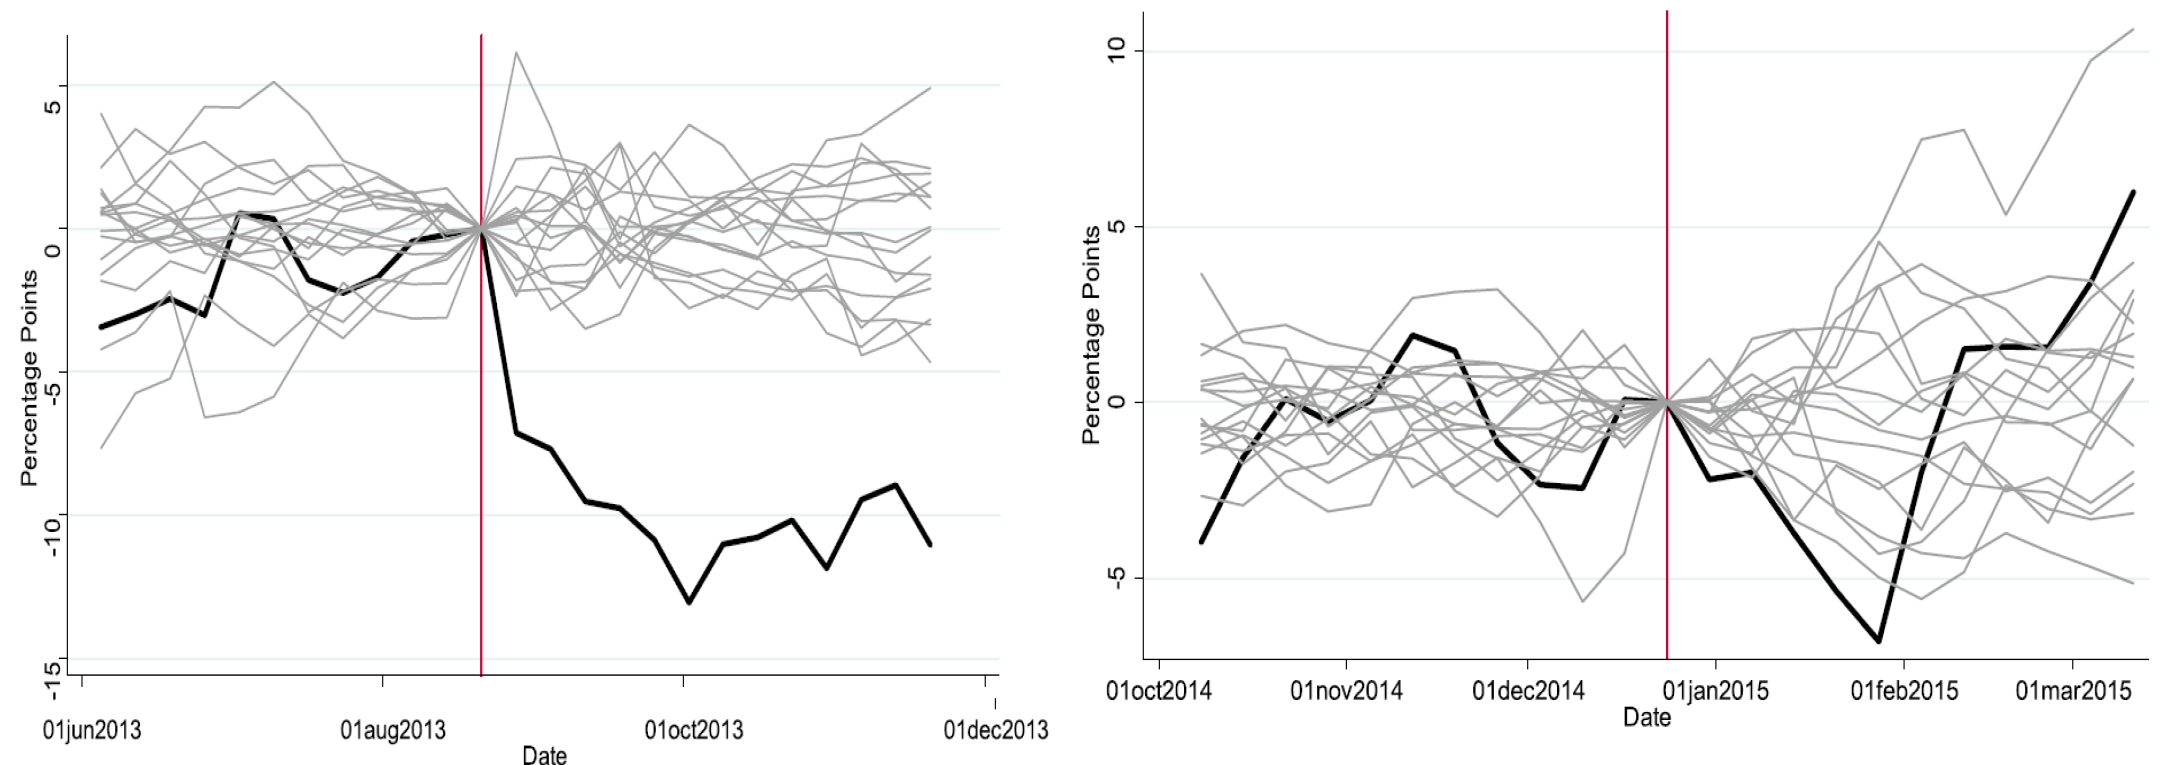
\includegraphics[width=0.75\paperwidth]{img/brazil_two_interventions_effects.PNG}}
  \medskip
  \emph{Source: Gonzalez, Khametshin, Peydro and Polo (2019)}

  
\end{frame}


\subsection{Colombia}

\begin{frame}
  \frametitle{Colombia Call and Put Options to Hedge Volatility Risk}
  \begin{wideitemize}
    \item Objective: mitigate FX volatility, after the shift to a flexible exchange rate regime in 1998/99 (used to be crawling bands). \emph{"Offer to the market hedges against extreme circumstances"}
    \item Offer \textbf{put} (protection against depreciation) and \textbf{call} (protection against appreciation) \textbf{options}
      \begin{itemize}
      \item TRM: representative market Colombian peso/US dollar exchange rate
      \item Strike prices: +5\% Higher (put) or -5\% lower (call) than the 20-day moving average of the TRM 
      \item Threshold takes into account a low probability of activation, due to the +/- 5\% limit
      \item Amount fixed at USD 180 million then USD 200 million
      \end{itemize}
    \item Some discretion was applied: 
      \begin{itemize}
      \item When the Colombian peso was weak, the central bank deactivate the put, because the central bank didn't want to buy USD at this price.
      \item Added some discretion when high demand (threshold, etc.)
      \end{itemize}      
  \end{wideitemize}
\end{frame}

\begin{frame}
\frametitle{Colombian Central Bank Foreign Exchange Interventions 1999-2017}
\makebox[\linewidth]{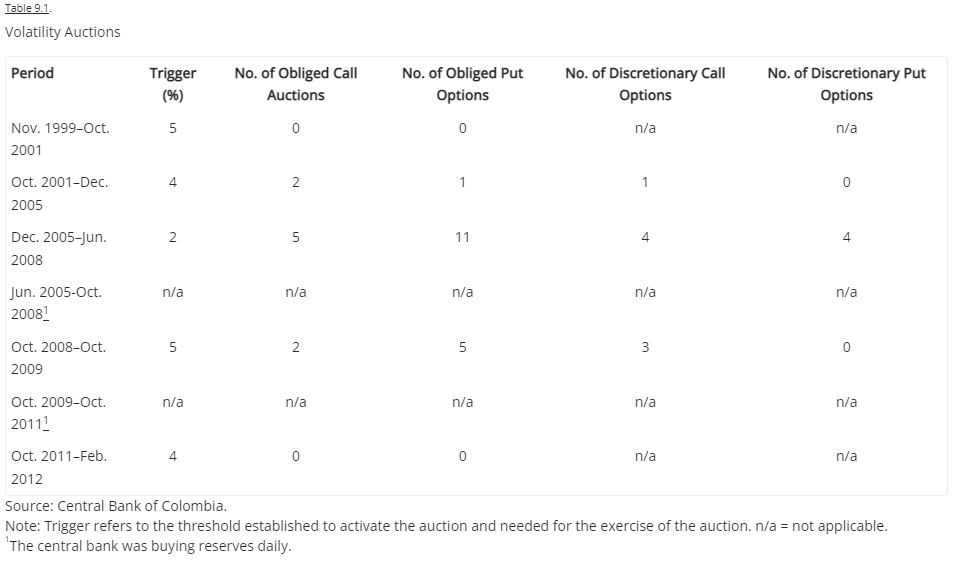
\includegraphics[width=0.7\paperwidth]{img/colombia_options_table.PNG}}
\medskip
\emph{Source: Cardozo (2019)}
\end{frame}

\begin{frame}
  \frametitle{Colombia: Put Options to Accumulate USD Reserves}
  \begin{wideitemize}
    \item How to accumulate FX reserves at the best price and limiting market impact?
    \item Following Mexico's experience, the Colombian central bank auctioned these options at the end of each month (1999-2002 and 2003-2008) to banks, financial corporations and the MoF
    \item USD options with \textbf{one-month maturity} and a \textbf{strike price equal to the representative market Colombian peso/US dollar exchange rate (TRM)}
    \item Agents can only exercise the option when the TRM was below the 20-day average
      \begin{itemize}
      \item The central bank could then avoid buying US dollar when the Colombian peso is weaker than the previous 20 days
      \end{itemize}      
  \end{wideitemize}
\end{frame}


\begin{frame}
  \frametitle{Colombia Put Options to Accumulate USD Reserves}

  \begin{wideitemize}
    \item Suitable approach to accumulate FX reserves while minimizing market impact
    \item Through these auctions, the central bank bought USD 3.4 billion in 8 years
      \begin{itemize}
      \item All 49 auctions were oversubscribed, with min/max amount of USD 30 million and USD 250 million
      \end{itemize}
  \end{wideitemize}

\end{frame}


\begin{frame}
\frametitle{Colombian Central Bank Foreign Exchange Interventions 1999-2017}
\makebox[\linewidth]{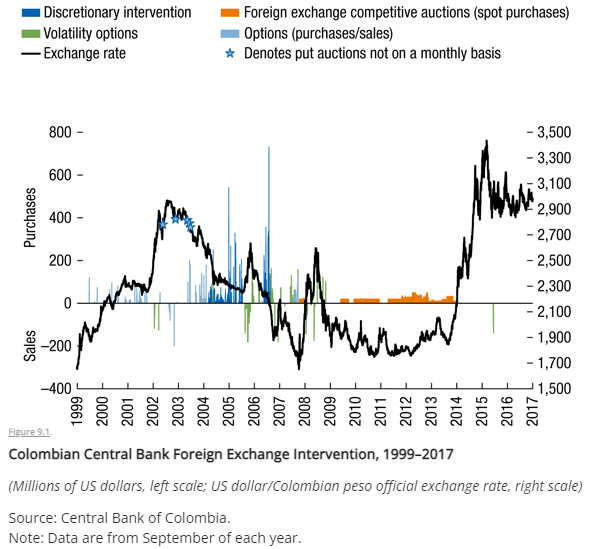
\includegraphics[height=0.6\paperheight]{img/colombia_put_options.PNG}}
\medskip
\emph{Source: Cardozo (2019)}
\end{frame}


\begin{frame}
  \frametitle{Selling Reserves for Preserving Financial Stability}
  \begin{wideitemize}
    \item Colombia is an inflation targeter operating a flexible exchange rate regime
    \item Foreign interventions should therefore be motivated by financial stability concerns
    \item The operating procedure depends on the type of financial stability threats
      \begin{itemize}
      \item If financial agents suffer from \textbf{closure in FX credit lines}: the central bank intervenes through \textbf{FX swaps} and acts as a liquidity provider
        \begin{itemize}
        \item \emph{FX swaps don't transfer FX risks}
        \end{itemize}        
      \item If there is no private provision of FX hedge on the market, the central bank steps in and provide \textbf{USD non-deliverable forwards}
        \begin{itemize}
        \item \emph{FX forwards do transfer FX risk}
        \end{itemize}
      \item If the foreign reserves are enough, sell spot. If not, sell USD NDF (settled in local currencies) 
      \end{itemize}
  \end{wideitemize}
\end{frame}


\begin{frame}
\frametitle{Decision Tree for Selling Reserves}
\makebox[\linewidth]{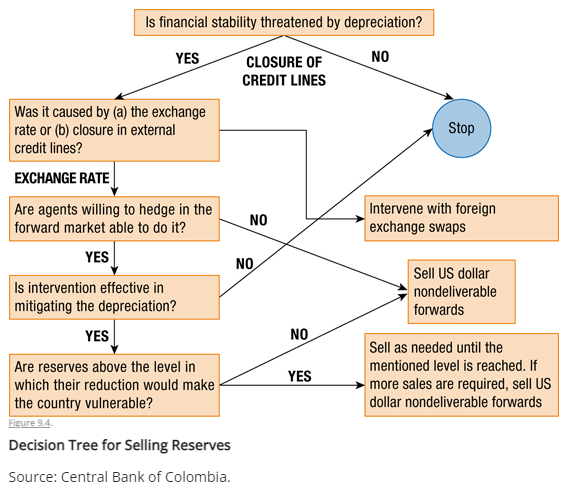
\includegraphics[height=0.6\paperheight]{img/colombia_decision_tree.PNG}}
\medskip
\emph{Source: Central Bank of Colombia}
\end{frame}

\subsection{Thailand}

\begin{frame}
  \frametitle{Thailand BOT FXI Objectives}
  According to the BOT-BIS article \href{https://www.bis.org/publ/bppdf/bispap104x.pdf}{\beamergotobutton{link}}, the objectives of the BOT are:
  \begin{wideitemize}
    \item Curtail excessive and persistent volatility
    \item Discourage speculation
    \item Deter sharp capital flows
    \item Not intended to influence the exchange rate level, nor gaining competitiveness
  \end{wideitemize}
\end{frame}


\begin{frame}
  \frametitle{BOT FXI Implementation}

  \begin{wideitemize}
    \item Uses both verbal and actual interventions
    \item Discretionary timing based on "market developments and market conditions" (volatility, liquidity, etc.)
      \begin{itemize}
      \item Looking not only at the spot against USD but also the NEER, the REER and other regional currencies
      \end{itemize}
    \item Conducted mainly via USD/THB spot on both onshore and offshore markets
    \item The BOT employs a designated agent to maintain anonymity in the market
      \begin{itemize}
      \item Cancel the signaling effect 
      \item Yet the BoT is highly credible, with more than USD 225 bn FX reserves in 2023
      \end{itemize}
  \end{wideitemize}  
\end{frame}


\begin{frame}
  \frametitle{BOT Sterilization}
  \begin{wideitemize}
  \item Main instruments: BOT bills and bonds (54\%)
    \begin{itemize}
    \item Main instrument, supporting market development and curve pricing
    \item 14-day to three-year maturity
    \item Separate segments with the Ministry of Finance to avoid arbitrages
    \end{itemize}
    \item Bilateral repurchase operations and deposit faciliy (30\%)
    \item FX swaps (16\%)
      \begin{itemize}
      \item Absorb THB while injecting USD in up to one-years tenors
      \item Mostly used to alleviate USD funding costs in Thailand
      \end{itemize}
      
  \end{wideitemize}
\end{frame}

\begin{frame}
\frametitle{BOT: Total Absorption Instruments Outstanding}
\makebox[\linewidth]{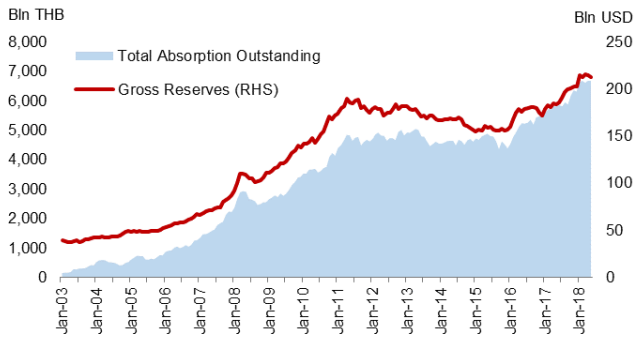
\includegraphics[width=0.75\paperwidth]{img/thailand_sterilization.PNG}}
\medskip
\emph{Source: Bank of Thailand (2018)}
\end{frame}


\begin{frame}
  \frametitle{BOT Communication}
  \begin{wideitemize}
  \item The BOT doesn't announce interventions ex-ante nor ex-post
  \item Consistent with the market anonymity it is looking for
  \item Yet, it publishes its level of foreign reserves weekly with one-week lag
   \item Direct comunications regarding the effect of FX policy and market operations are also addressed to key influencers - researchers, private analysts and members of the press -
      \begin{itemize}
      \item who in turn will make their own communication to the general public
      \end{itemize}
  \end{wideitemize}
\end{frame}






%% ---------------------------------------------------------------------------
%% End document
%% ---------------------------------------------------------------------------
\end{document}


%% ---------------------------------------------------------------------------
%% Sample code
%% ---------------------------------------------------------------------------

% \begin{frame}
% \frametitle{Example with a Figure}
%     \makebox[\linewidth]{\includegraphics[width=\paperwidth]{../output/step_007_top_ae_dotplot.pdf}}
% \end{frame}


% \begin{frame}
% \begin{adjustwidth}{-2em}{-2em} % Wider frame 
%   \frametitle{Example with a Wide Table}  
%   \setlength\tabcolsep{4pt}  % default value: 6pt
%   %\footnotesize
%   \centering
%   \input{../output/mytable.tex}\\
% \end{adjustwidth}
% \end{frame}









%%% Local Variables:
%%% mode: latex
%%% TeX-master: t
%%% End:


%%% Local Variables:
%%% mode: latex
%%% TeX-master: t
%%% End:
